\documentclass[a4paper,12pt,numbers=noenddot]{scrreprt}
\usepackage[left= 3cm,right = 3cm, bottom = 3cm, top = 3cm]{geometry}
\usepackage[onehalfspacing]{setspace}

% ============= Settings for the document =============
\def\workTitle{HST Project S5}
\def\subTitle{CircuitVoyager Pre1}
\def\studentFirstNameone{Joel}
\def\studentLastNameone{Schaller}
\def\advisorPreTitle{}
\def\advisoFirstName{Enrico}
\def\advisorLastName{Malacarne}
\def\advisorPosTitle{}
\def\dateDay{22}
\def\dateMonth{09}
\def\dateYear{2023}


% ============= Packages =============

% Switch between German and English such as the title page design based on the main.tex. file settings
\usepackage{ifthen}


\usepackage[english]{babel} % English


% Standard Packages
\usepackage[utf8]{inputenc}
\usepackage{graphicx} % Used to insert images
\usepackage{float} %Package for using the [H] option on graphics to force them into place
\usepackage[export]{adjustbox} % Used to constrain images to a maximum size
\usepackage{enumerate} % Needed for markdown enumerations to work
\usepackage{geometry} % Used to adjust the document margins
\usepackage{amsmath} % Equations
\usepackage{amssymb} % Equations
\usepackage[mathletters]{ucs} % Extended unicode (utf-8) support
\usepackage{fancyvrb} % verbatim replacement that allows latex
\usepackage{grffile} % extends the file name processing of package graphics
\usepackage{url}
\def\UrlBreaks{\do\/\do-}
\usepackage{hyperref}
\usepackage{longtable} % longtable support required by pandoc >1.10
\usepackage{multicol}
\usepackage{multirow}
\usepackage[nohyperlinks]{acronym}
\usepackage{enumitem}
\usepackage{fixmath}
\usepackage{blindtext}
\usepackage[T1]{fontenc}
\usepackage{graphicx}
\usepackage{subfigure}
\graphicspath{{Figures/}} % define path of images
\usepackage{animate}
\usepackage{fancyhdr}
\usepackage{lmodern}
\usepackage[dvipsnames]{xcolor}
\usepackage{footnote}
\usepackage{lastpage}

\usepackage{pgfgantt}

% Citation style
\bibliographystyle{ieeetr}

% BlockDiagram Drawing Package
\usepackage{tikz}
\usetikzlibrary{shapes,arrows}
\usepackage[european,nooldvoltagedirection]{circuitikz}
\usepackage{pgfplots}
\pgfplotsset{compat=1.10}
\usepackage{mathtools}
\usepackage{pgf-pie}
\usepackage{textcomp}
\usepackage{pgfplots}
\usepgfplotslibrary{statistics}
\usepackage{smartdiagram}

%  ============= BlockDiagram Drawing Config =============
% Definition of blocks:
\tikzset{%
  block/.style    = {draw, thick, rectangle, minimum height = 3em,
    minimum width = 3em},
  sum/.style      = {draw, circle, node distance = 2cm}, % Adder
  input/.style    = {coordinate}, % Input
  output/.style   = {coordinate}, % Output
  mult/.style	  = {draw, isosceles triangle, minimum height=1cm, minimum width =1cm}
}

%  ============= Settings for listings  =============
\usepackage{listings,lstautogobble}
\lstset{title=\lstname, frame=single, framerule=0pt, rulecolor=\color{lightgray}, showspaces=false, showstringspaces=false, showtabs=false, numbers=left, numbersep=5pt, numberstyle=\sffamily\tiny\color{gray}, breaklines=false, autogobble=true, basicstyle=\sffamily\scriptsize}

\usepackage[breakable]{tcolorbox}
\newtcolorbox{codeblock}{
    colback=gray!5!white,
    colframe=gray!95!black,
    before skip=20pt,
    after skip=20pt
    }
\newtcolorbox{codeblock-b}{
    breakable,
    colback=gray!5!white,
    colframe=gray!95!black,
    before skip=20pt,
    after skip=20pt
    }
\newtcolorbox{box-black}{
    colback=black,
    colframe=black,
    before skip=10pt,
    after skip=10pt
    }

%  ============= Color definition ============= 
% FH-Blau
\definecolor{FH}{RGB}{8, 64, 126}
\definecolor{FH2}{RGB}{8, 64, 126}

% ============= No massive space betweend headline and chapter titel =============
\renewcommand*{\chapterheadstartvskip}{\vspace*{-.4cm}}
\renewcommand*{\chapterheadendvskip}{\vspace{.5cm}}

\setlength{\parindent}{0pt} % no indent at paragraph start

% ============= Header and Footer =============
\renewcommand{\chaptermark}[1]{\markboth{\thechapter~ #1}{}}

\fancypagestyle{icmt-fancy}{%
  \fancyhf{}% Clear header and footer
  %\fancyhead[L]{\leftmark}
  \fancyhead[L]{\subTitle}
  \fancyhead[R]{\dateDay.\dateMonth.\dateYear}
  \fancyfoot[L]{\studentFirstNameone~\studentLastNameone}
  \fancyfoot[C]{TBZ / ETHZ}
  \fancyfoot[R]{\thepage}% Custom footer *~|~\pageref{LastPage}
  \renewcommand{\headrulewidth}{0.4pt}% Line at the header visible
  \renewcommand{\footrulewidth}{0.4pt}% Line at the footer visible
}

% Define horizontal lines above and below the main content
\makeatletter
\def\thickhline{%
	\noalign{\ifnum0=`}\fi\hrule \@height \thickarrayrulewidth \futurelet
	\reserved@a\@xthickhline}
\def\@xthickhline{\ifx\reserved@a\thickhline
	\vskip\doublerulesep
	\vskip-\thickarrayrulewidth
	\fi
	\ifnum0=`{\fi}}
\makeatother
\newlength{\thickarrayrulewidth}
\setlength{\thickarrayrulewidth}{2\arrayrulewidth}

% ============= Redefine the plain page style =============
\fancypagestyle{plain}{%
  \fancyhf{}%
  \fancyfoot[R]{\thepage}%
  \renewcommand{\headrulewidth}{0.0pt}% Line at the header invisible
  \renewcommand{\footrulewidth}{0.0pt}% Line at the footer visible
}
\renewcommand*{\chapterpagestyle}{icmt-fancy}

% ============= Size of headings =============
\setkomafont{chapter}{\LARGE}
\setkomafont{section}{\Large}
\setkomafont{subsection}{\large}
\setkomafont{subsubsection}{\normalsize}
\setkomafont{paragraph}{\normalsize}
\setkomafont{subparagraph}{\small}

% roman numbering with \RM{Zahl}
\newcommand{\RM}[1]{\MakeUppercase{\romannumeral #1}}

% ============= hyperref should always be added at the end =============
\usepackage{hyperref}

\hypersetup{
    unicode=false, % non-Latin characters in Acrobat’s bookmarks
    pdftoolbar=true, % show Acrobat’s toolbar?
    pdfmenubar=true, % show Acrobat’s menu?
    pdffitwindow=true, % window fit to page when opened
    pdfstartview={FitV}, % fits the width of the page to the window
    pdfpagelayout={SinglePage}, % displays only one page when opened in pdf viewer
    pdftitle={\workTitle},
	pdfsubject={\subTitle},
	pdfauthor={\studentFirstNameone~\studentLastNameone},
	pdfkeywords={\workTitle,~\subTitle},
    pdfcreator={pdflatex}, % creator of the document
    pdfproducer={LaTeX with hyperref}, % producer of the document
    pdfnewwindow=true, % links in new window
    colorlinks=false, % false: boxed links; true: colored links
    linkcolor=black, % color of internal links (change box color with linkbordercolor)
    citecolor=black, % color of links to bibliography
    filecolor=black, % color of file links
 	breaklinks=true,	
	menucolor=black,
    urlcolor=black % color of external links
}


% ============= Begin of the main document =============
\begin{document}
% Title Page will change automatic

\newgeometry{left=2.4cm,right=2.4cm,bottom=2.5cm,top=2cm}

% first titlepage
\pagestyle{empty}

\begin{center}
\vspace{2cm}

\centering
\Huge{{\color{FH2}{\fontsize{24}{30} \textbf{\sffamily{\workTitle}}\\}}}
\LARGE{{\color{FH2}{\fontsize{16}{24} \textbf{\sffamily{\subTitle}}\\}}}
\vspace{2cm}



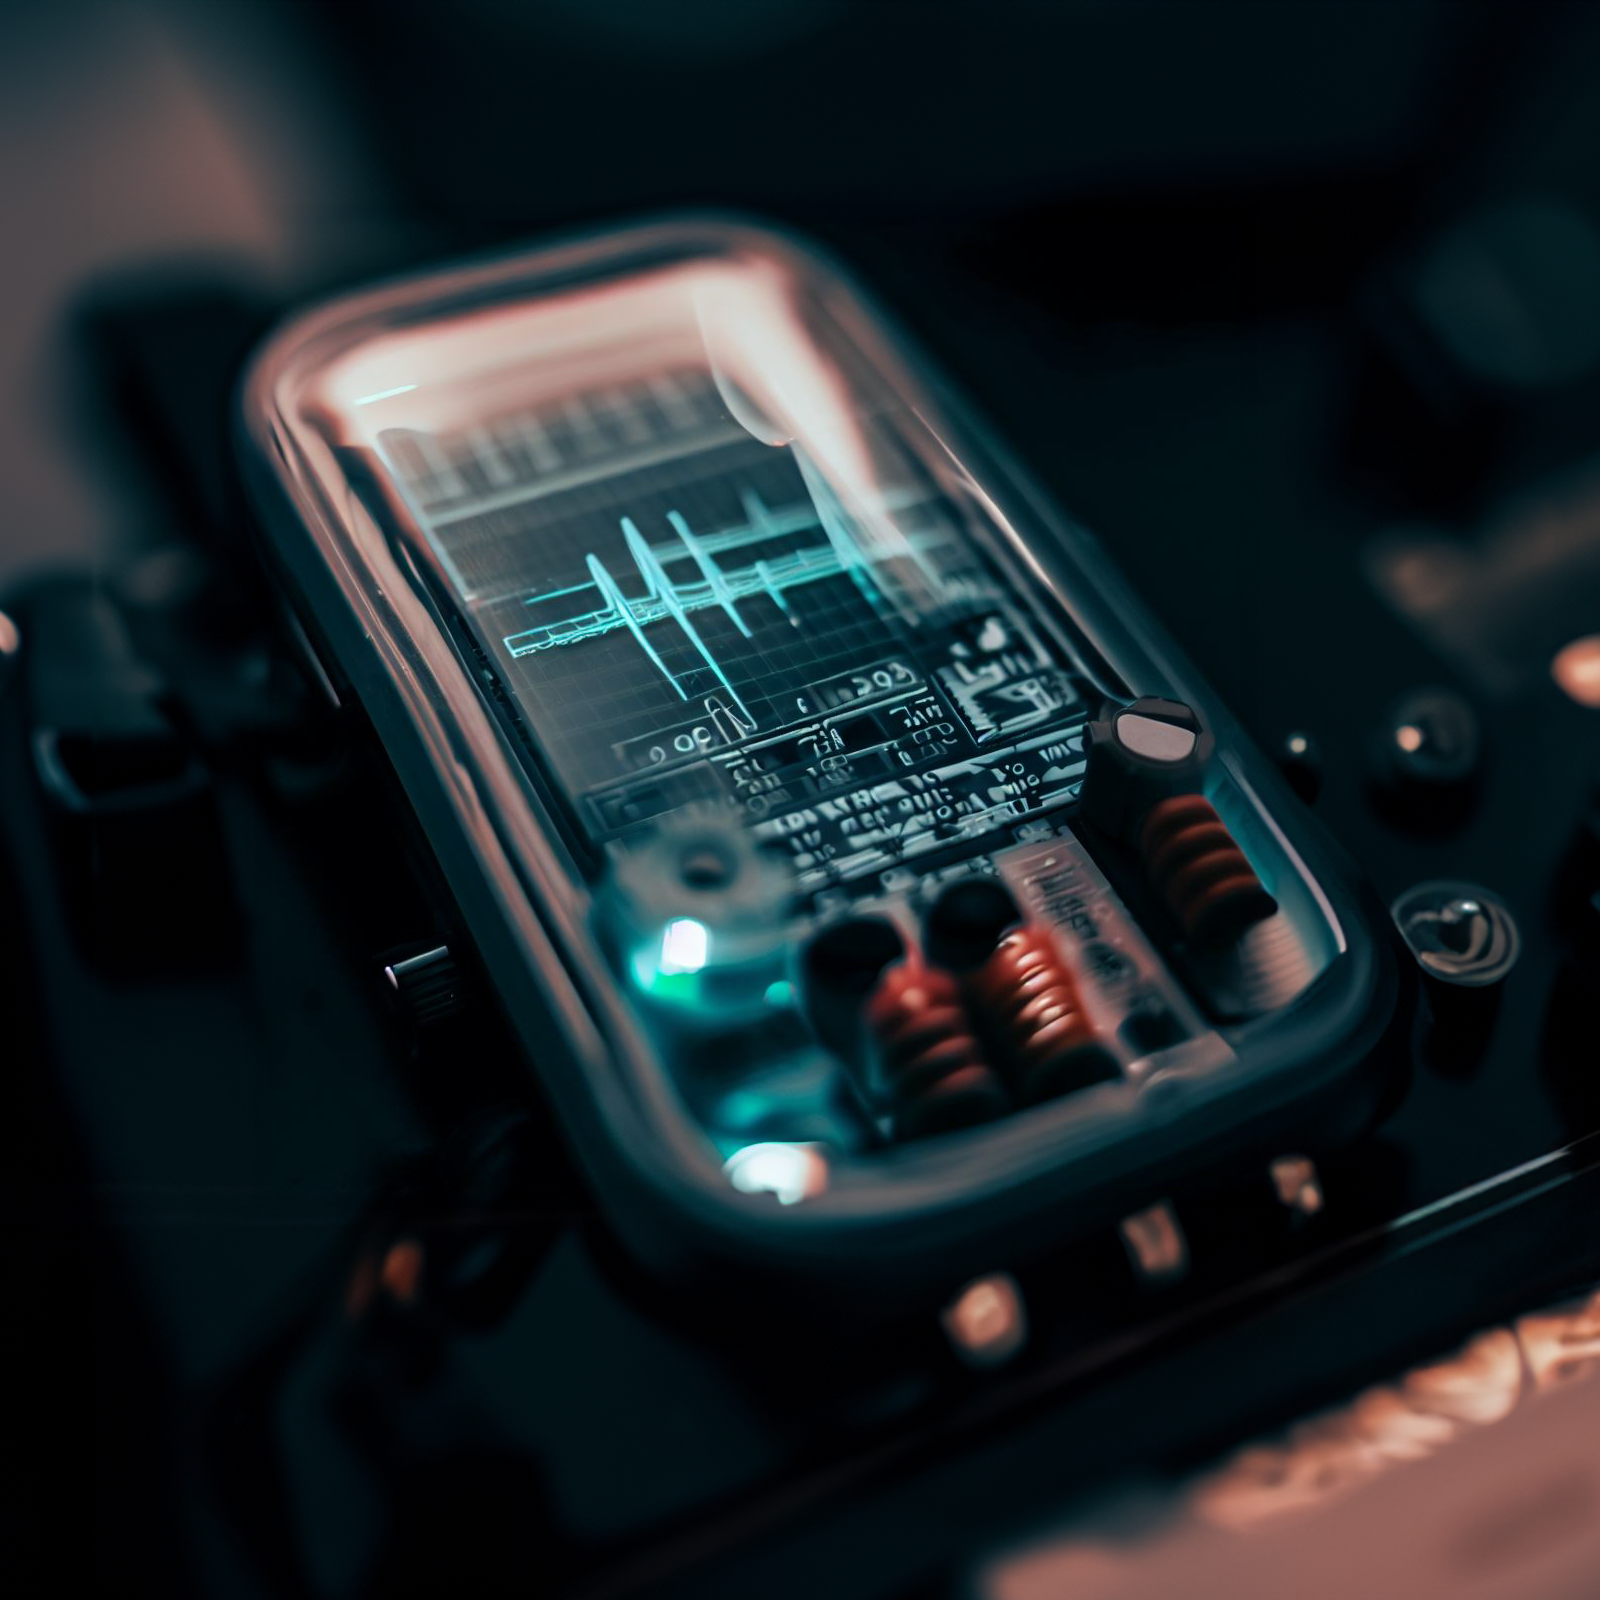
\includegraphics[width=16cm]{Resources/Pictures/title.png}


\vfill

\large
Submitted by:\\
\fontsize{15pt}{15pt}\selectfont
\textbf{\sffamily{\studentFirstNameone\ \studentLastNameone}} \\
\fontsize{11pt}{15pt}\selectfont

\vspace{0.8cm}

\begin{tabular}{lll}
Lecturer: \advisoFirstName\ \advisorLastName\\
\end{tabular}

\vspace{0.8cm}

\normalsize{\dateDay.\dateMonth.\dateYear}


\end{center}

\restoregeometry

\pagenumbering{Roman} % roman page numbering

\chapter*{Abstract}
\textit{
\\ Konzept (gestalterisch) 
\\ Methode  
\\ Wichtigste Ergebnisse
}
\cleardoubleemptypage

% Table of content
\setcounter{tocdepth}{1} % Levels in the table of content
\tableofcontents
\cleardoubleemptypage
\pagenumbering{arabic} % arabic page numbering

\setlist[enumerate,1]{label*=\arabic*.,font=\bfseries\sffamily}

\pagestyle{icmt-fancy}
% ================================
% =            CONTENT           =
% ================================
\chapter{Introduction}
\label{cha:Introduction}
\textit{Vorstellung von Thema und eigenem gestalterischen Konzept oder Konstruktionsplan in Bezug auf das Oberthema, Darlegung der Motivation für die Arbeit, Erläuterung der verwendeten Methoden, Überblick über den schriftl. Kommentar}
\chapter{Main Body}
\label{cha:Main Body}


\section{''Pflichtenheft''}
\label{sec:Pflichtenheft}

\subsubsection{Cost}
I've already bought two \acs{devboard}s one of them stays at \acs{tbz} and the other is at home. One of these boards was paid by Mr. Malacarne. Further expenses from the \acs{pcb} will be paid by me and shouldn't exceed about 50 CHF, as the \acs{hw} isn't that complicated.

\subsubsection{Time}
The most time of the project I will work at home because it's a rather big project to execute in one semester. I will also have much time in the fall holidays to work on it. The project will approximately take 100h to complete. Also the more detailed timeplan is in chapter: [\ref{sec:GANTT Chart}]

\subsubsection{Tools}
To realize this project I will mainly use, the \acs{sw} STM32CubeIDE with \acs{hal}, STM32 CubeProgrammer and Altium Designer. The documentation is written in LaTeX in VSCode. And I'm planning to order the PCB on JLCPCB and I will populate and reflow the PCB at ETHZ, where I'm also allowed to use the measurement equipment for the HW tests.

\subsubsection{Technical Details}
\begin{table}[H]
    \centering
    \label{tab:Technical Details}
\begin{tabular}{||c || c | c | c | c  || c ||} 
 \hline
 value &  min. & typ. & max. & unit & description \\ [0.5ex] 
 \hline\hline
  supply voltage & & 5 & & V & over USB \\ 
 \hline
 curent to measure & 0 & & 1 & A & \\ 
 \hline
 voltage to measure & 0 & & 10 & V & \\ 
 \hline
\end{tabular}
    \caption{Technical Details}
\end{table}

\newpage


\section{Extension PCB}
\label{sec:Extension PCB}



\subsection{STMod+}
Interface from DevBoard to Extension PCB. 

\begin{itemize}
    \item 5V Supply
    \item SPI 
    \item I\textsubscript{2}C
    \item ADC
    \item Interrupt
    \item PWM
    \item GPIOs
\end{itemize}

I will use the STMOD\#14 connection that was intended to use as PWM, as a second ADC input. To measure current and voltage at the same time to later show the power cosumption of the DUT.

\begin{figure}[H]
	\centering
	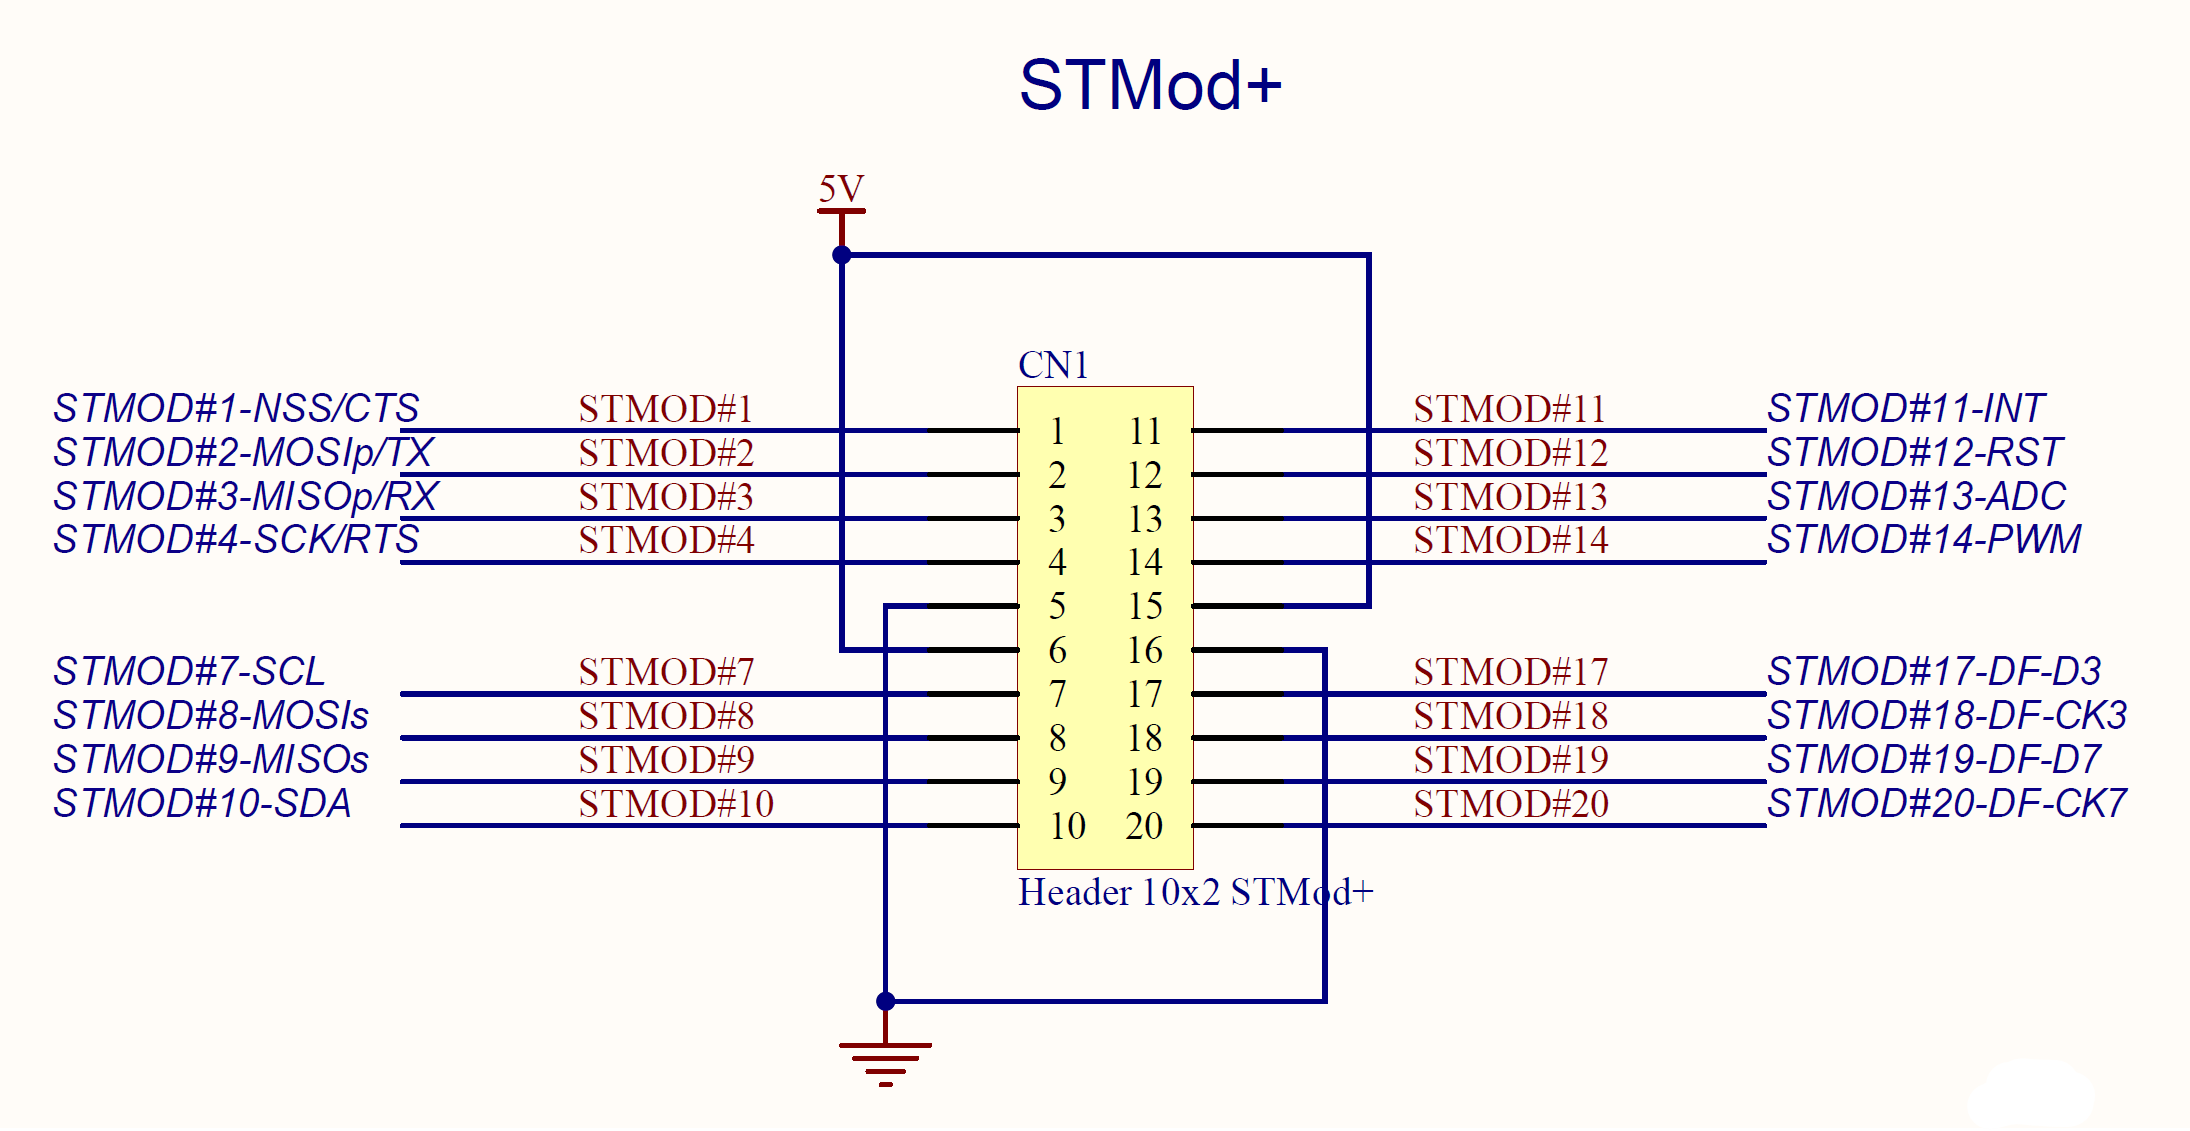
\includegraphics[width=13cm]{Resources/STMOD_Interface.png}
	\caption{STMod+ Interface}
	\label{fig:STMod+ Interface}
\end{figure}




\newpage

\subsection{Hardware concept}

After some thoughts I came up with the following HW concept.


\begin{figure}[H]
	\centering



    \tikzstyle{block} = [draw, fill=white, rectangle, 
    minimum height=3em, minimum width=6em]
    \tikzstyle{sum} = [draw, fill=white, circle, node distance=1cm]
    \tikzstyle{input} = [coordinate]
    \tikzstyle{output} = [coordinate]
    \tikzstyle{pinstyle} = [pin edge={to-,thin,black}]

    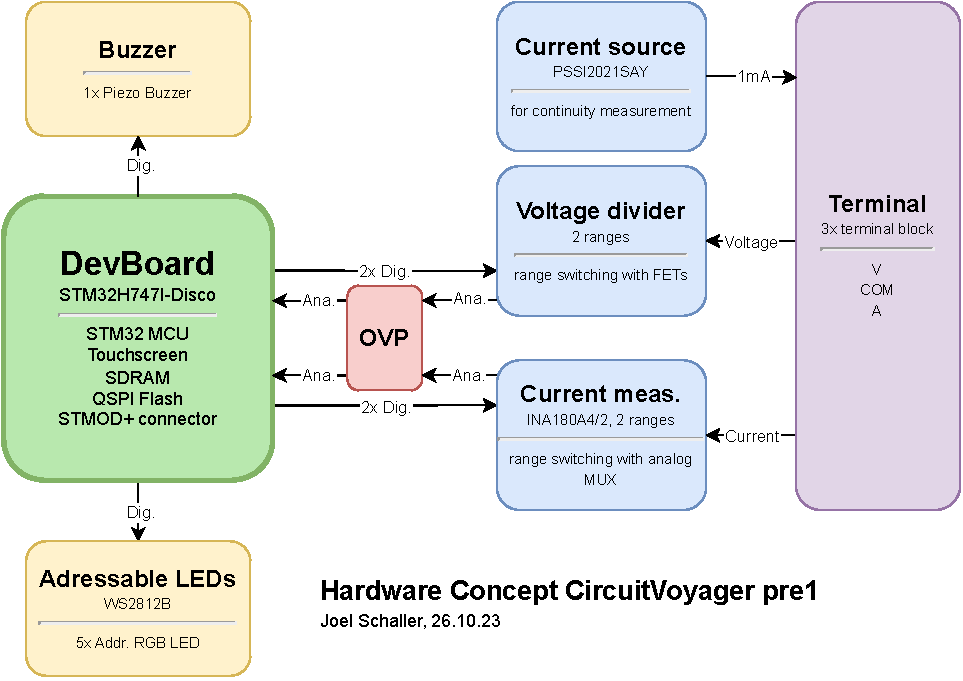
\includegraphics[width=15cm]{../../2_Project_Planning/HW_Concept/Hardware_Concept_CircuitVoyager_pre1.pdf}

    \vspace{0.2cm}

	\caption{Extension PCB HW concept}
	\label{fig:Extension PCB HW concept}
\end{figure}

\subsubsection{Voltage measurement}
To measure voltage, the DUT should be connected to the terminals V and COM. COM is connected internally to device GND. The V terminal is connected to the Voltage divider block. This block divides the input voltage down, so the ADC in the MCU doesn't overshoot. There are 2 ranges to measure voltage, which can be chosen by setting 2 digital output, that go from the MCU to the voltage divider. There's also an OVP, to protect the MCU from voltages higher than 3.3V. \cite{DMM_Video_ElectroNoobs}

\subsubsection{Current measurement}
To measure current, the DUT should be connected to the terminals A and COM. COM is connected internally to device GND. The A terminal is connected to current measurement block. This block measures the current, by letting the current flow through one of two shunt resistors. The DMM can choose which resistor and therefore range should be selected with the 2 digital Output that are connected from the MCU to the current measurement block. The voltage over the selected shunt is then amplified, by a current amplifier IC and then measured by the MCUs ADC. There's also an OVP, to protect the MCU from voltages higher than 3.3V. \cite{DMM_Video_ElectroNoobs}

\subsubsection{Continuity measurement}
To measure continuity, both the voltage divider and the current source is used. The continuity between the V and COM pins is measured. For this a constant current produced by the current source is flowing out of the V terminal. Simultaneously the voltage across those terminals is measured and the resistance / continuity can be evaluated. If continuity is detected, either the buzzer beeps or the LEDs blink. \cite{DMM_Video_ElectroNoobs}



\subsection{Schematic}
The schematic took me a bit longer than usual, because it's my first whole HW project in Altium before I used KiCAD and Altium is a lot more features and in my opinion is harder to learn. The schematic is in the Appendix \ref{sec:Extension PCB Schematics}.

\subsubsection{Buzzer Circuit}

\begin{figure}[H]
	\centering
	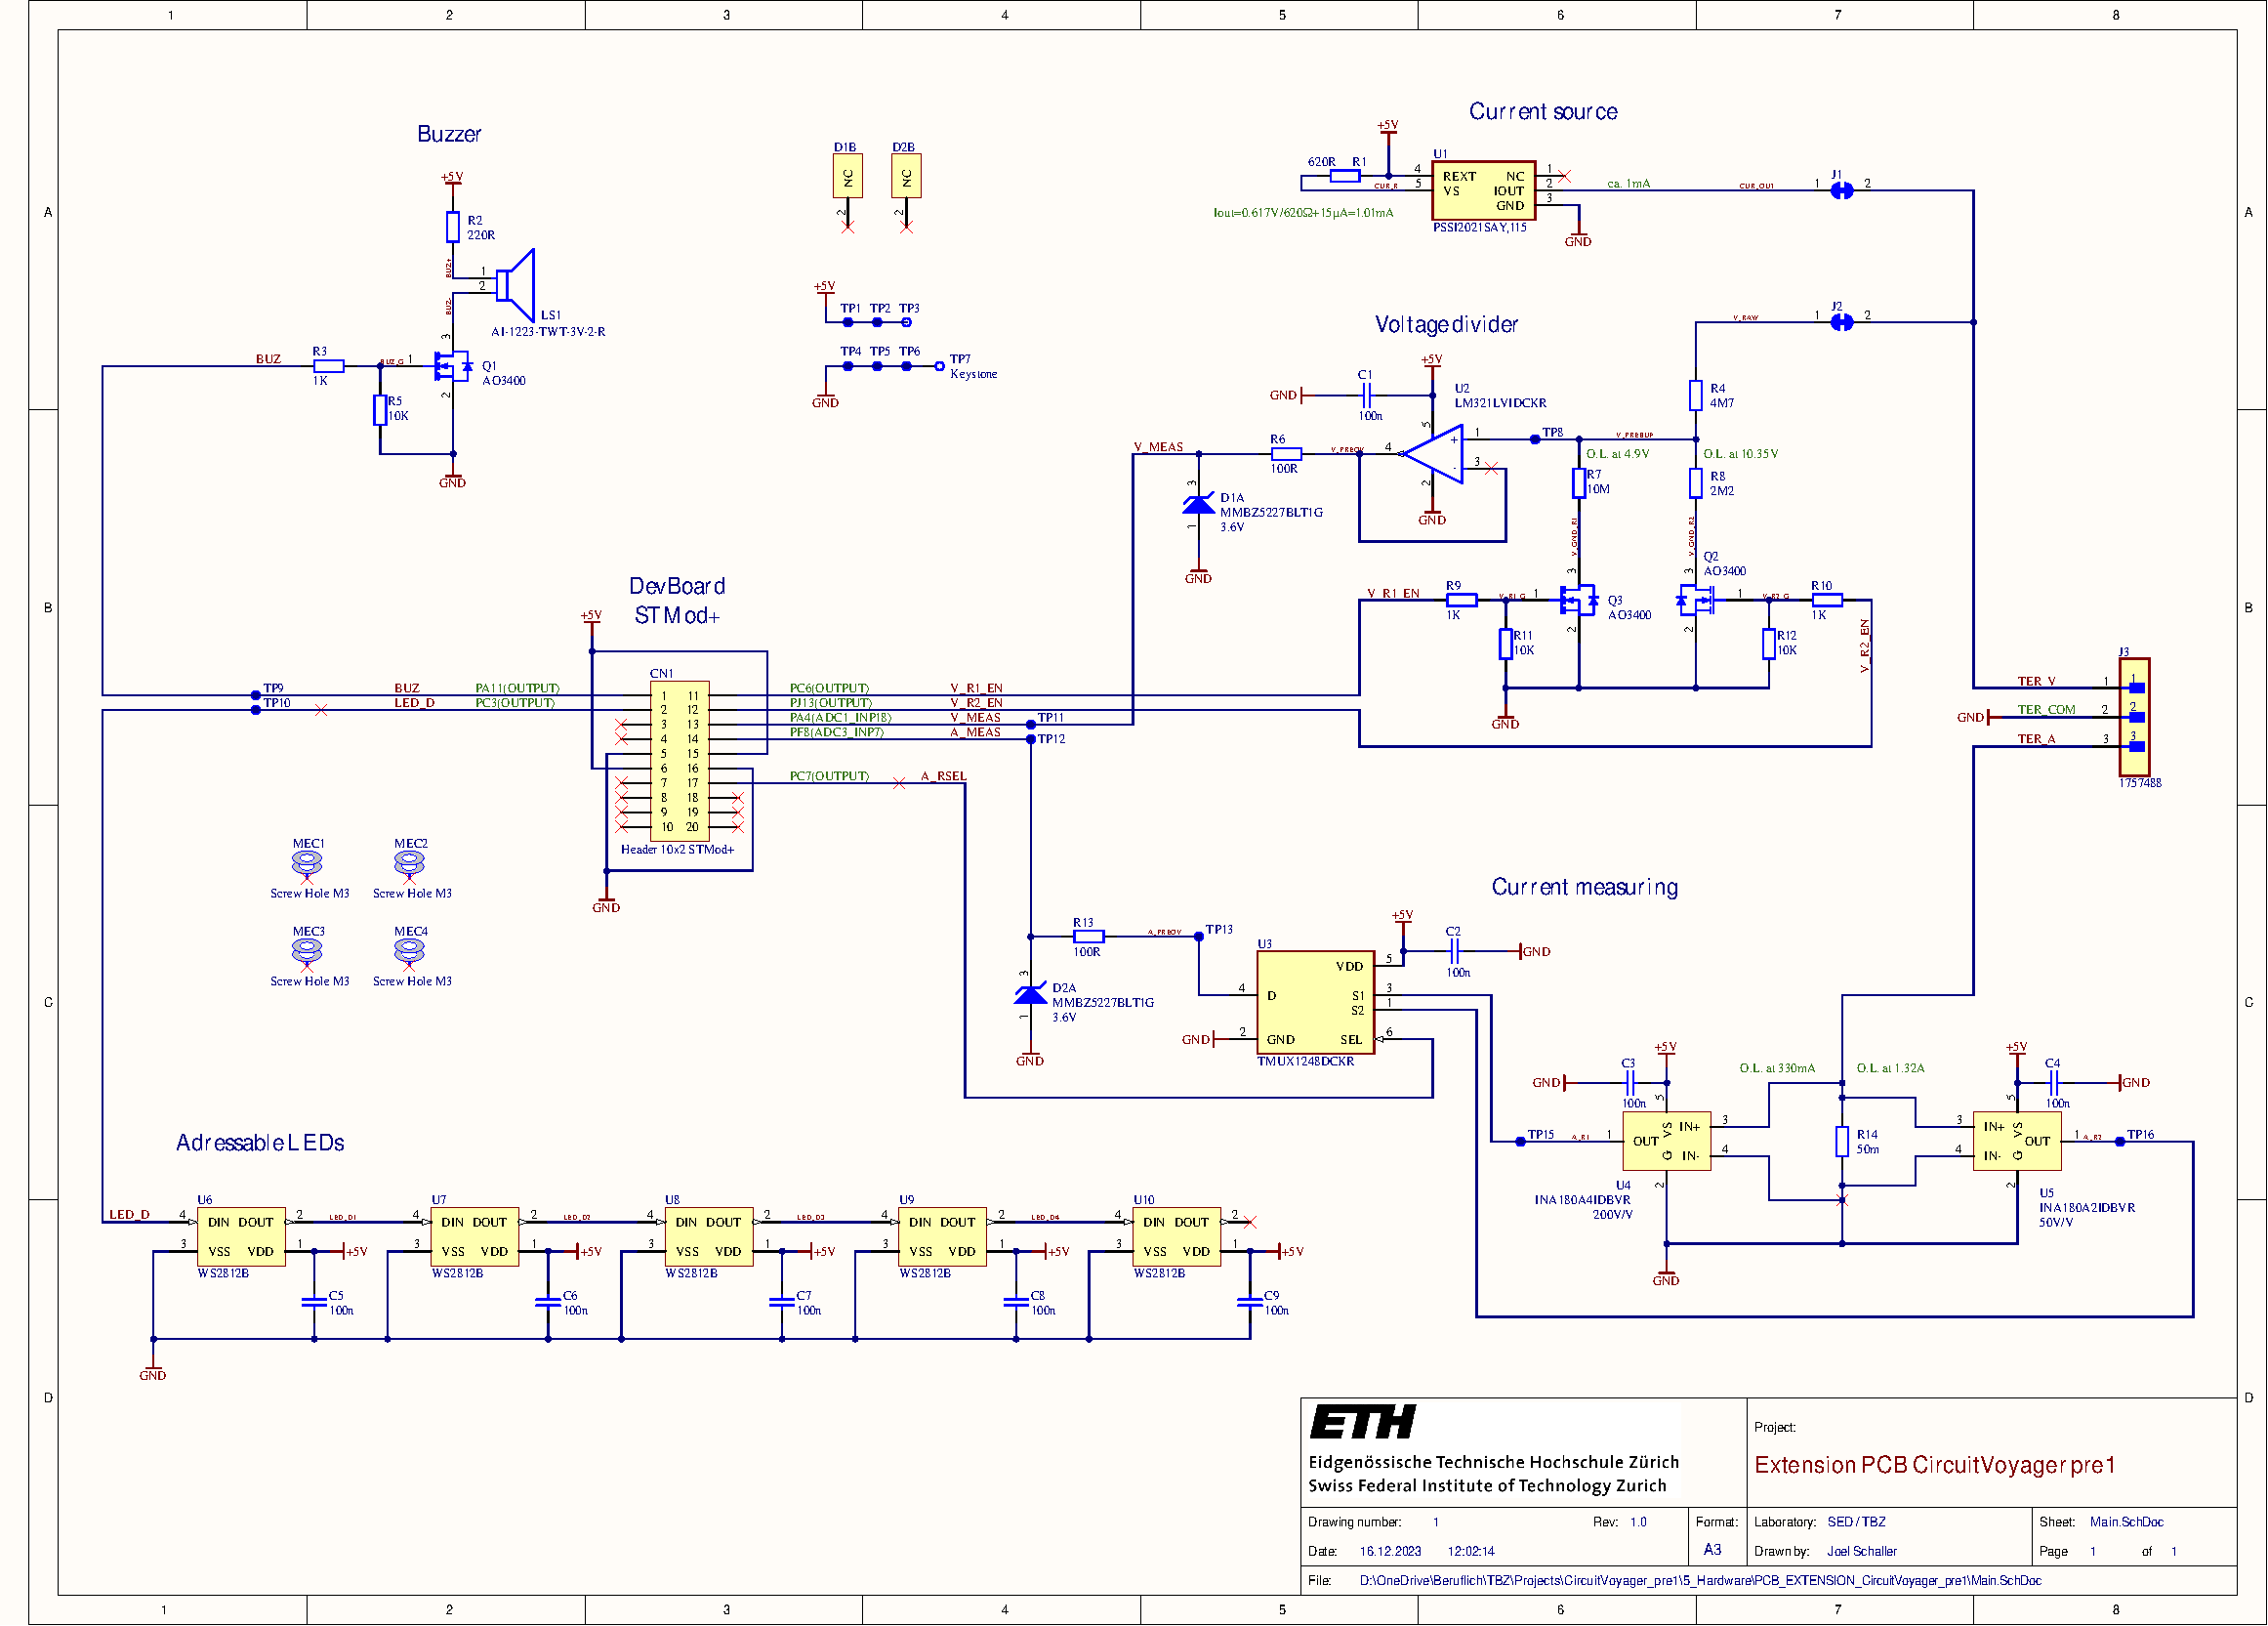
\includegraphics[width=8cm, trim={3.4cm 19cm 28.5cm 2cm}, clip]{../../../5_Hardware/PCB_EXTENSION_CircuitVoyager_pre1/Project Outputs for PCB_EXT_CV_PRE1/Schematic_PCB_EXTENSION_CircuitVoyager_pre1.pdf}
	\caption{Buzzer Circuit}
	\label{fig:Buzzer Circuit}
\end{figure}

This is an active buzzer. If the BUZ line is pulled high by the MCU, the MOSFET starts to conduct and the buzzer starts beeping. This circuit will be used to give an acoustic feedback to the user, if for example a continuity has been detected. 

The resistors R3 and R5 build a voltage divider with a ratio of 1/10. This has the advantage, that the gate capacitance of Q1 is charged with a limited current and if nothing's connected to the BUZ net the MOSFET turns the buzzer off and the whole machine isn't  in an indeterminate state.

The resistor R2 limit the current flowing through LS1. As LS1 is rated for 30mA at 3V.
\[R_2=\frac{U_{VCC}-U_{LS1}}{I_{LS1}}=\frac{5V-3V}{30mA}= \underline{\underline{66.\overline{6}\Omega}}\]

\[P_{R2}=I^2 \cdot R=(30mA)^2 \cdot 66. \overline{6} \Omega = \underline{\underline{60mW}}\]
Finally, I've chosen a 220\(\Omega\) resistor for R2. With this value the sound should be enough loud, that the user hears it. And the power loss of the resistor will be smaller. That means it should be perfectly fine to use a 0402 resistor that is rated for 62.5mW.


\subsubsection{Adressable LEDs Circuit}

\begin{figure}[H]
	\centering
	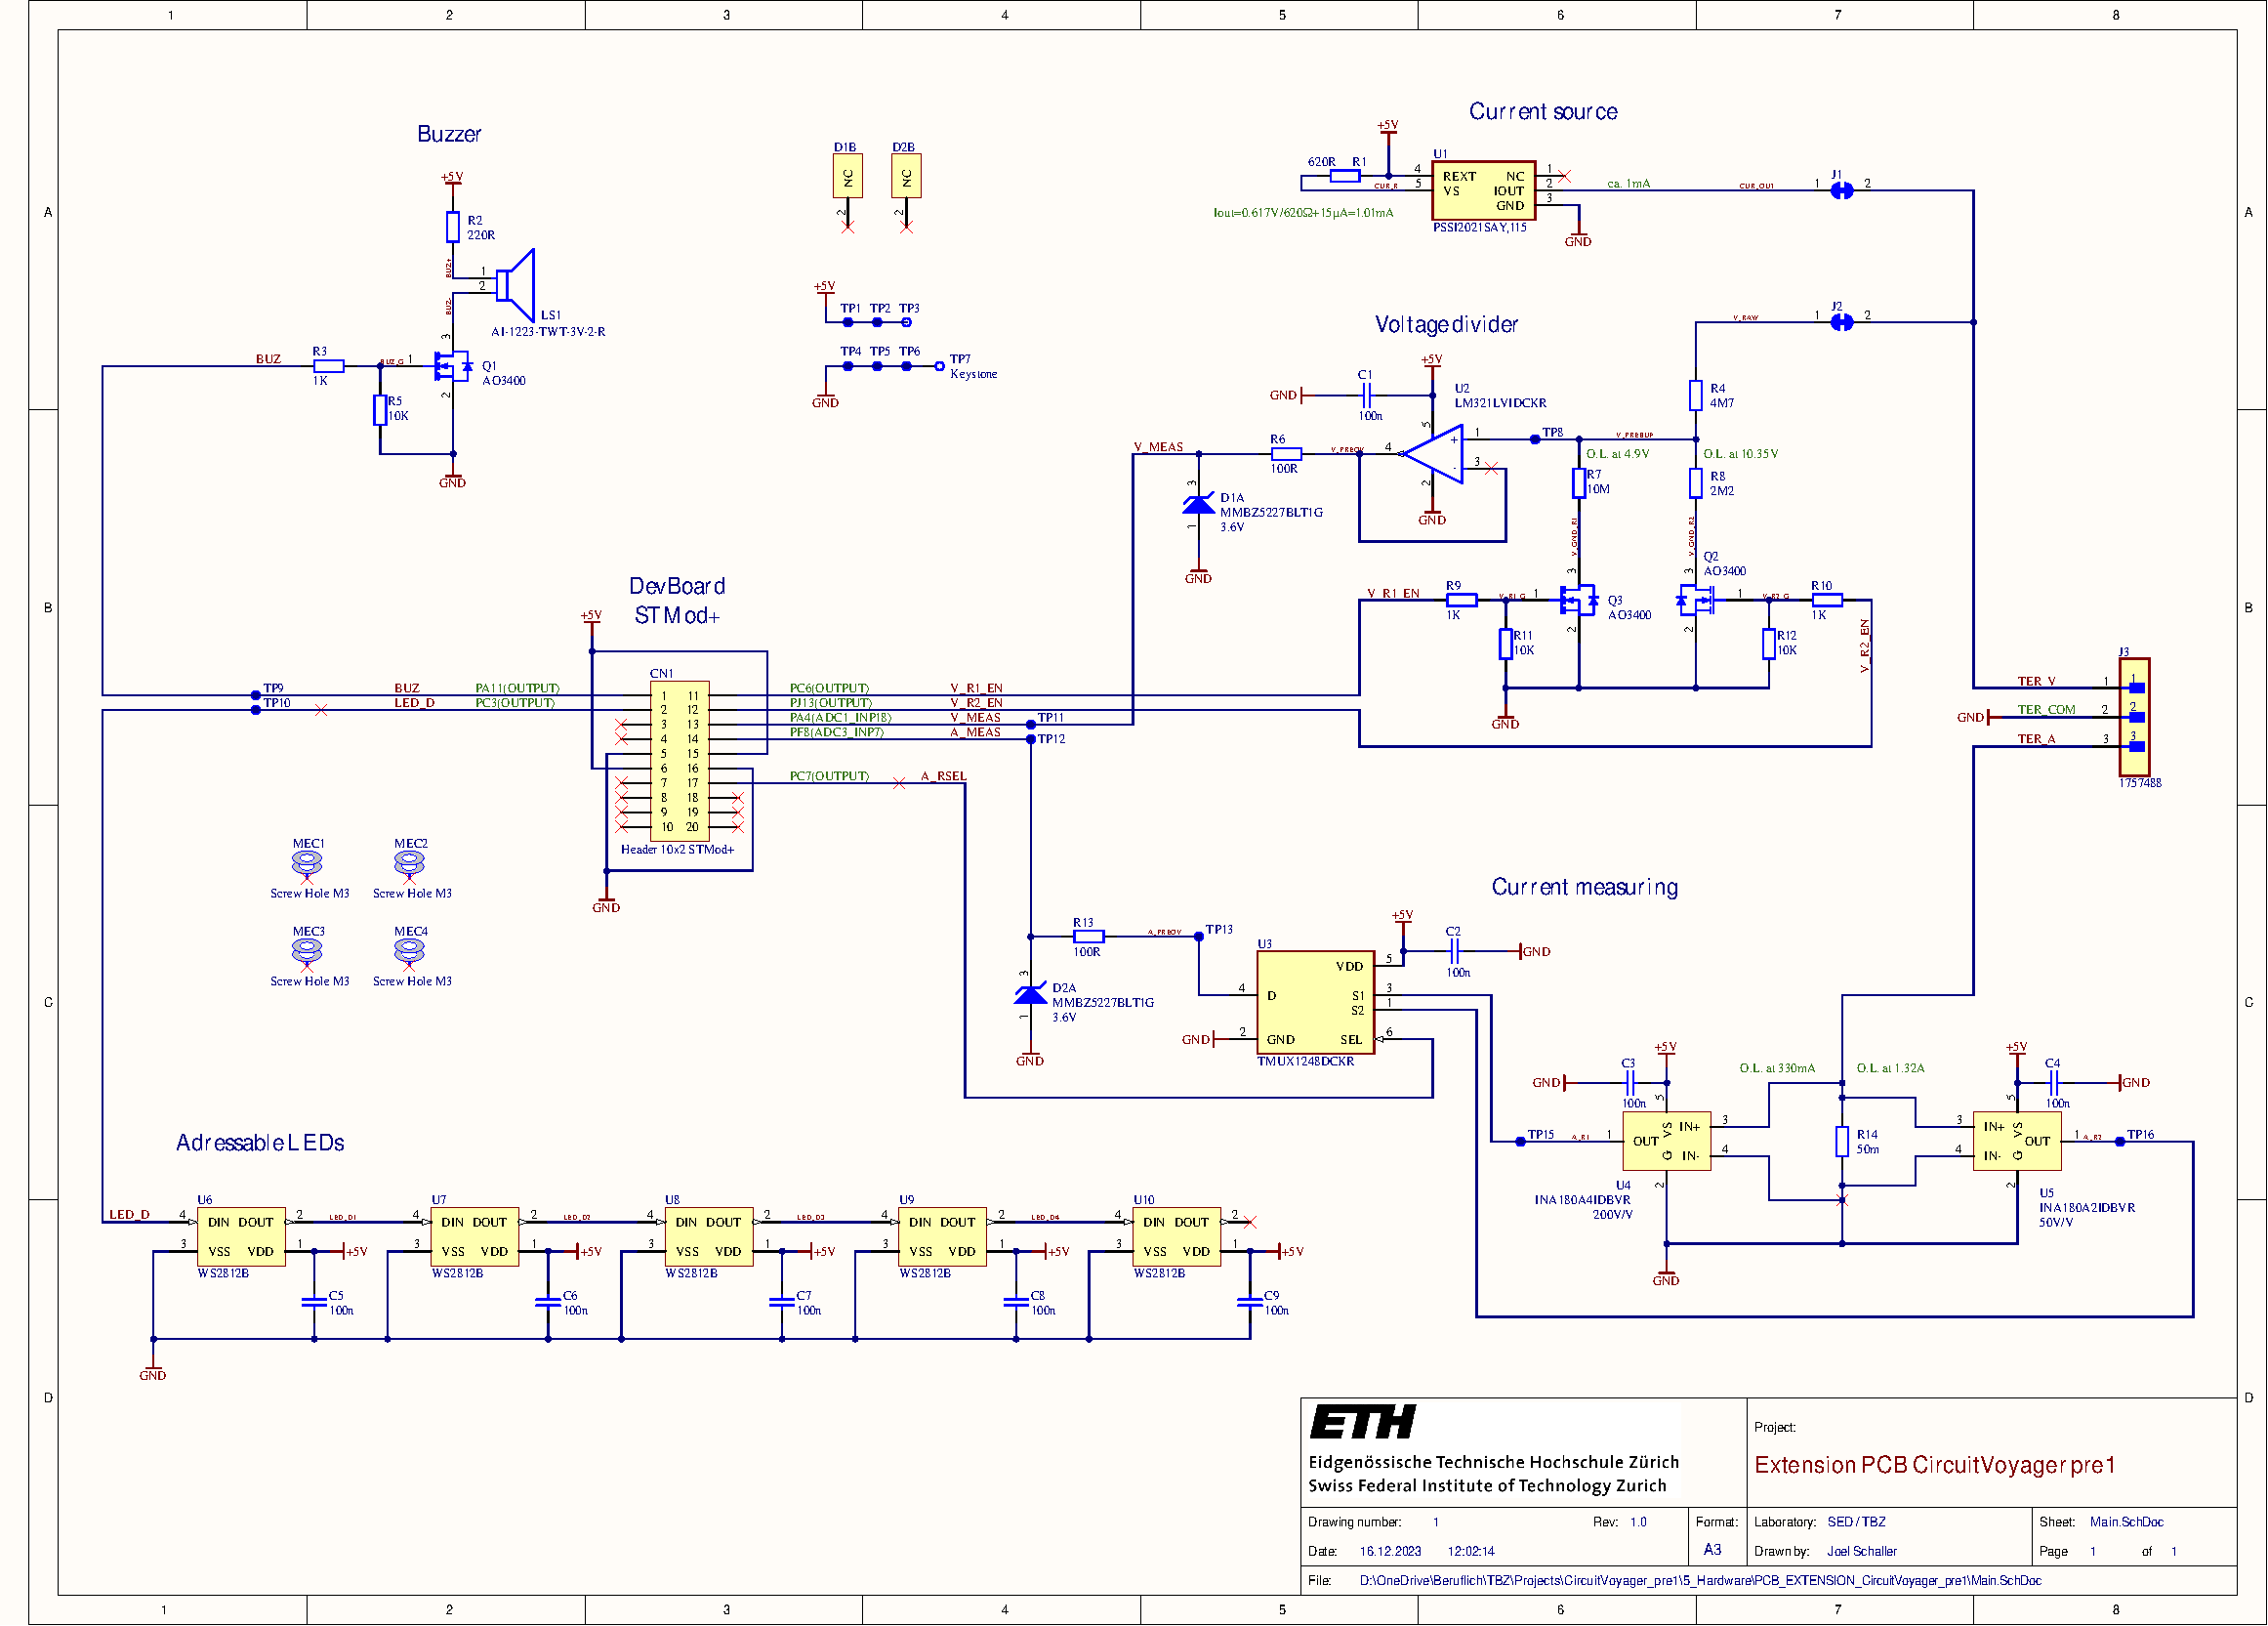
\includegraphics[width=15cm, trim={1.3cm 4cm 16.3cm 20cm}, clip]{../../../5_Hardware/PCB_EXTENSION_CircuitVoyager_pre1/Project Outputs for PCB_EXT_CV_PRE1/Schematic_PCB_EXTENSION_CircuitVoyager_pre1.pdf}
	\caption{Adressable LEDs Circuit}
	\label{fig:Adressable LEDs Circuit}
\end{figure}

An other option to show if continuity has been detected are these LEDs. The advantage of them is, that they only need one data connection and already include their logic and driving circuits. I've equiped the with one bulk C each, because they're integrated components and they're driven over the 5V rail, which they're specified for. But if they're driven by 5V they theoretically detect all voltages over 3.5V as a logical high. But the MCU only output 3.3V. I've used those LEDs much in past projects and this was never a problem, so I'm assuming that it should also work this time.



\subsubsection{Overvoltage Protection Circuit}

\begin{figure}[H]
	\centering
	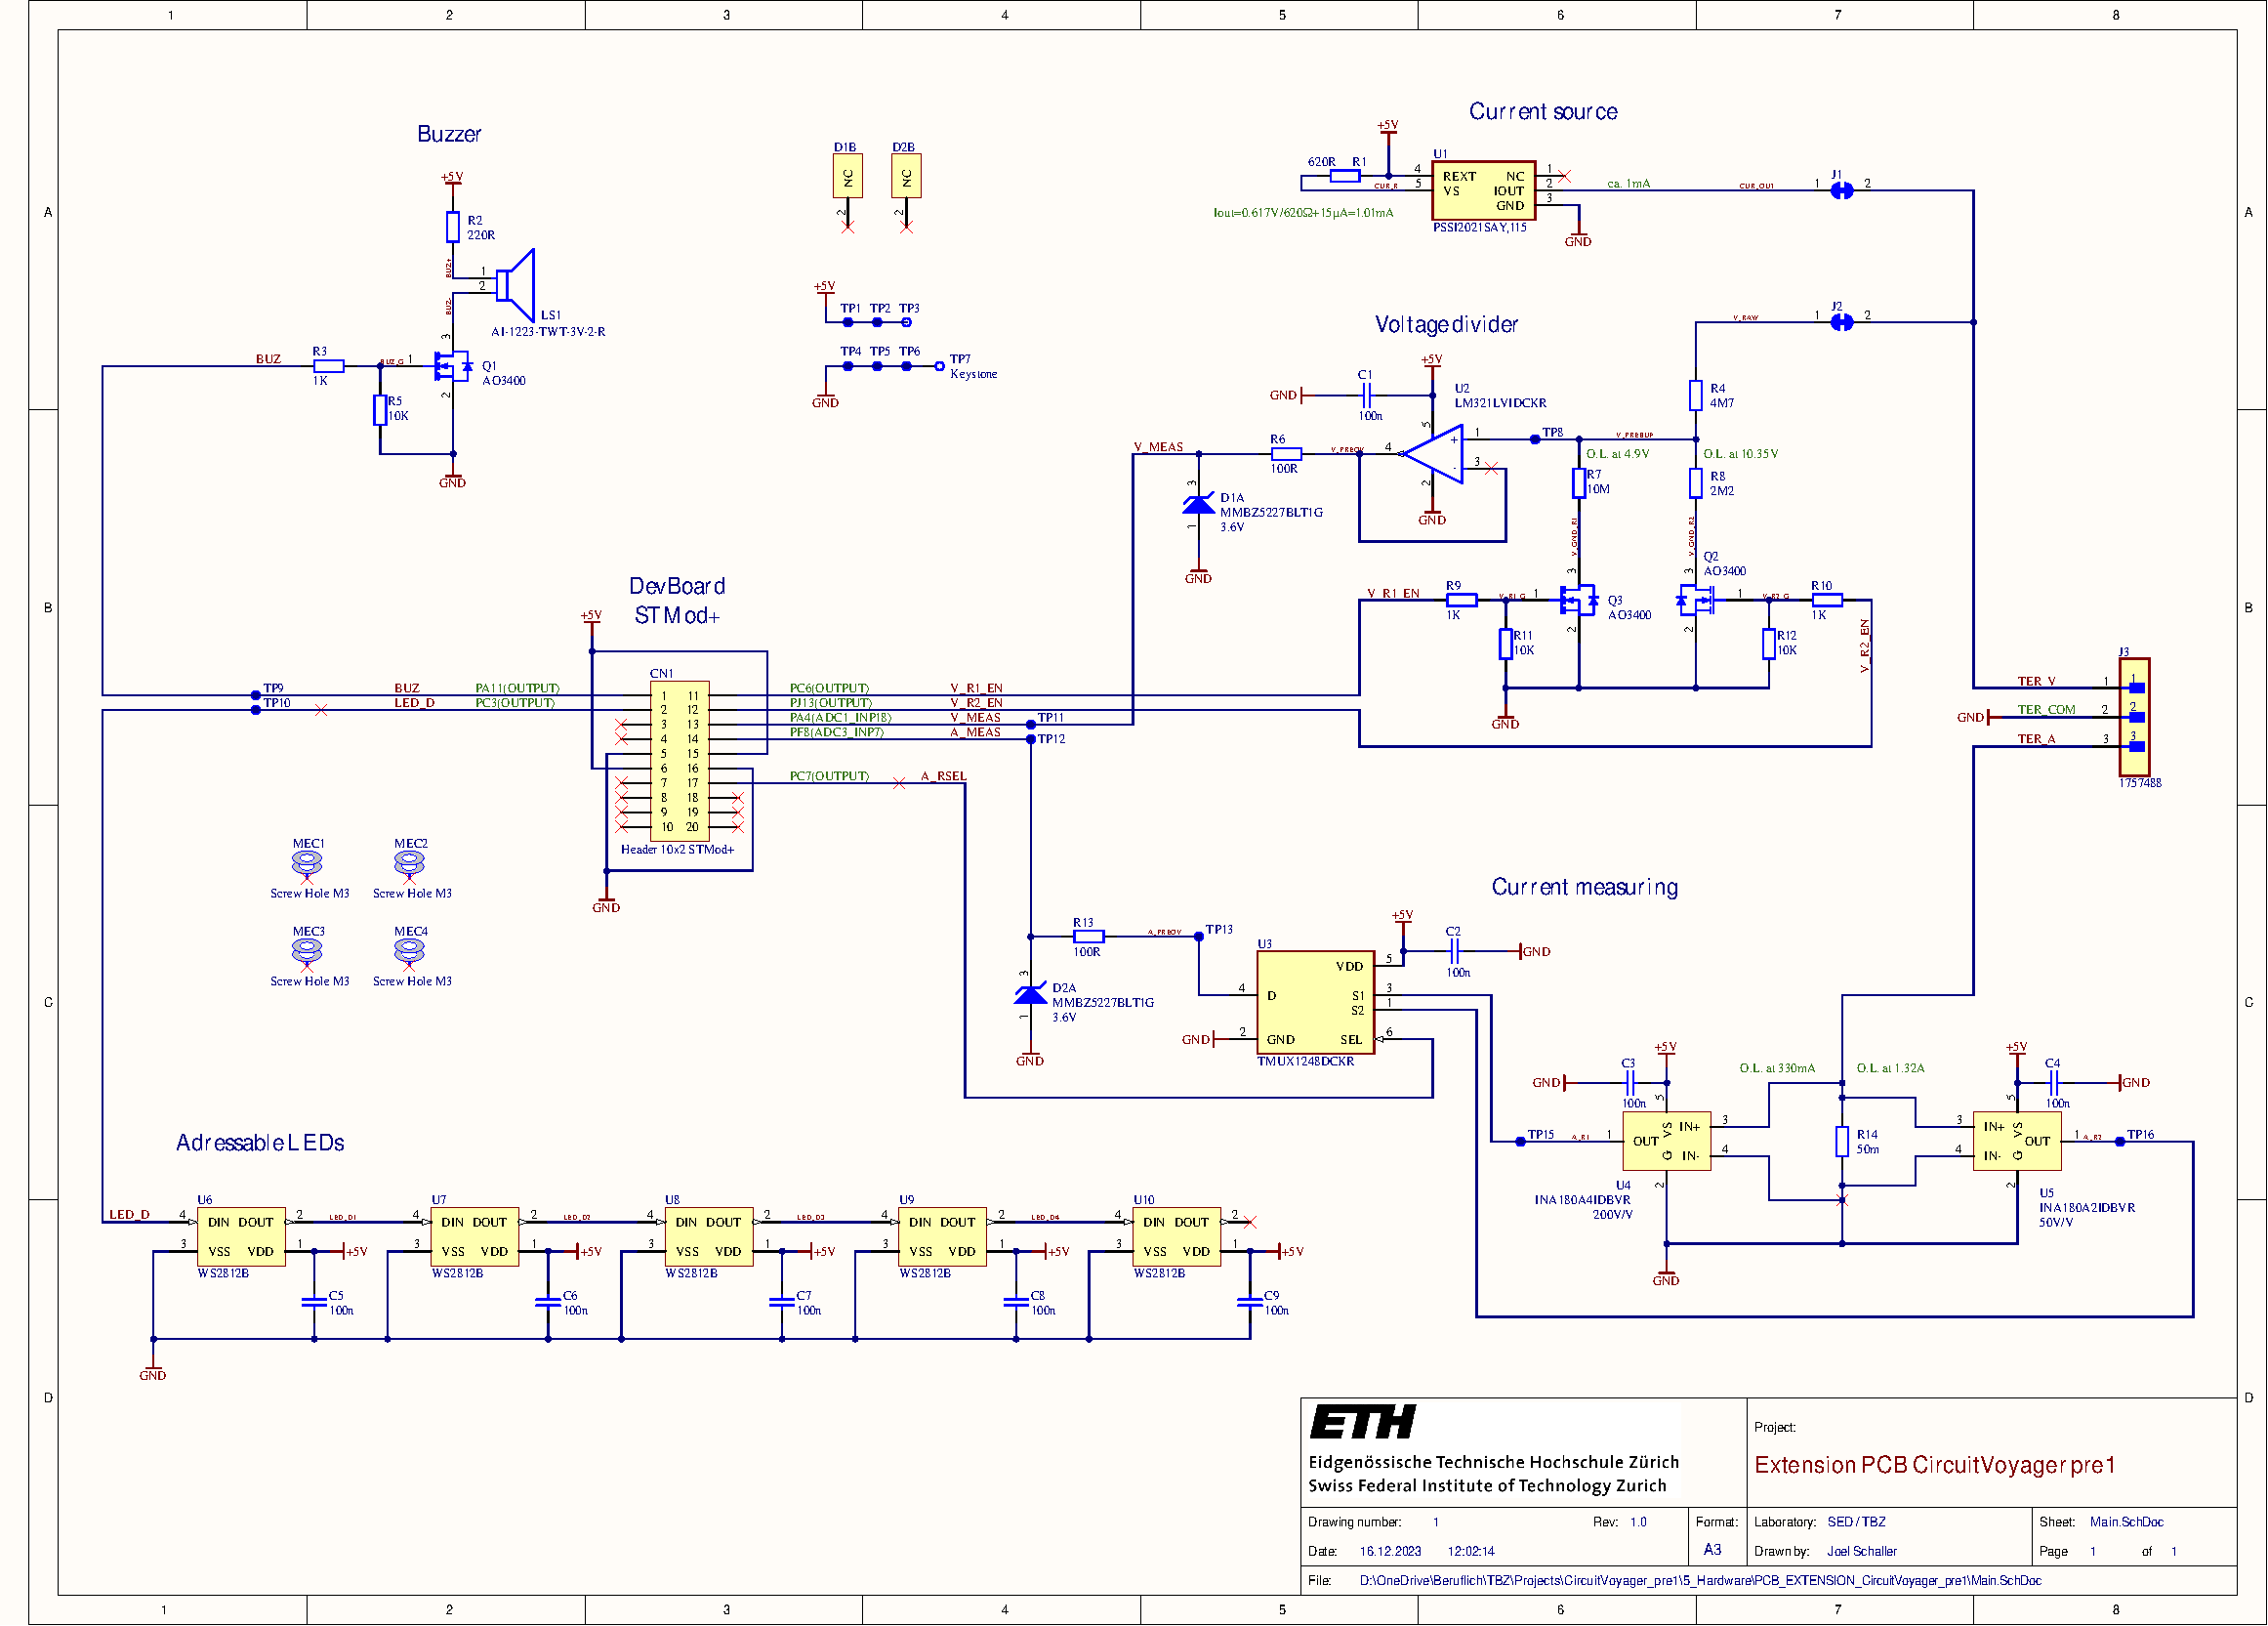
\includegraphics[width=6cm, trim={17cm 9.5cm 19cm 15.5cm}, clip]{../../../5_Hardware/PCB_EXTENSION_CircuitVoyager_pre1/Project Outputs for PCB_EXT_CV_PRE1/Schematic_PCB_EXTENSION_CircuitVoyager_pre1.pdf}
	\caption{Overvoltage Protection Circuit}
	\label{fig:Overvoltage Protection Circuit}
\end{figure}

My Problem is, that the voltages coming from  the Extension PCB, can't exceed 4V according to the MCUs datasheet. But because this PCB is powered by the 5V rail, theoretically these voltages could damage the MCU. So the goal was to develop a circuit which protects the ADC inputs. The first idea that came to my mind was to use varistors. I've already used the once in a project, but after reading some application notes on this topic, I decided to use a zenerdiode for the OVP. \cite{Protecting_ADC_Inputs_AN}

The zenerdiode I've used has a nominal zenervoltage of 3.6V (max. 3.78V) at 20mA. Together with R13 this should result with a maximum voltage of 3.78V at the ADC inputs. As long as the PREOV voltage doesn't exceed 5.6V.
\[U_{PREOV(MAX.)} = R_{13} \cdot I_Z + U_Z = 100\Omega \cdot 20mA + 3.6V = \underline{\underline{5.6V}}\]
\[P_{R13} = R \cdot I^2 = 100\Omega \cdot (20mA)^2 = \underline{\underline{40mW}}\]


\subsubsection{Voltage Divider Circuit}

\begin{figure}[H]
	\centering
	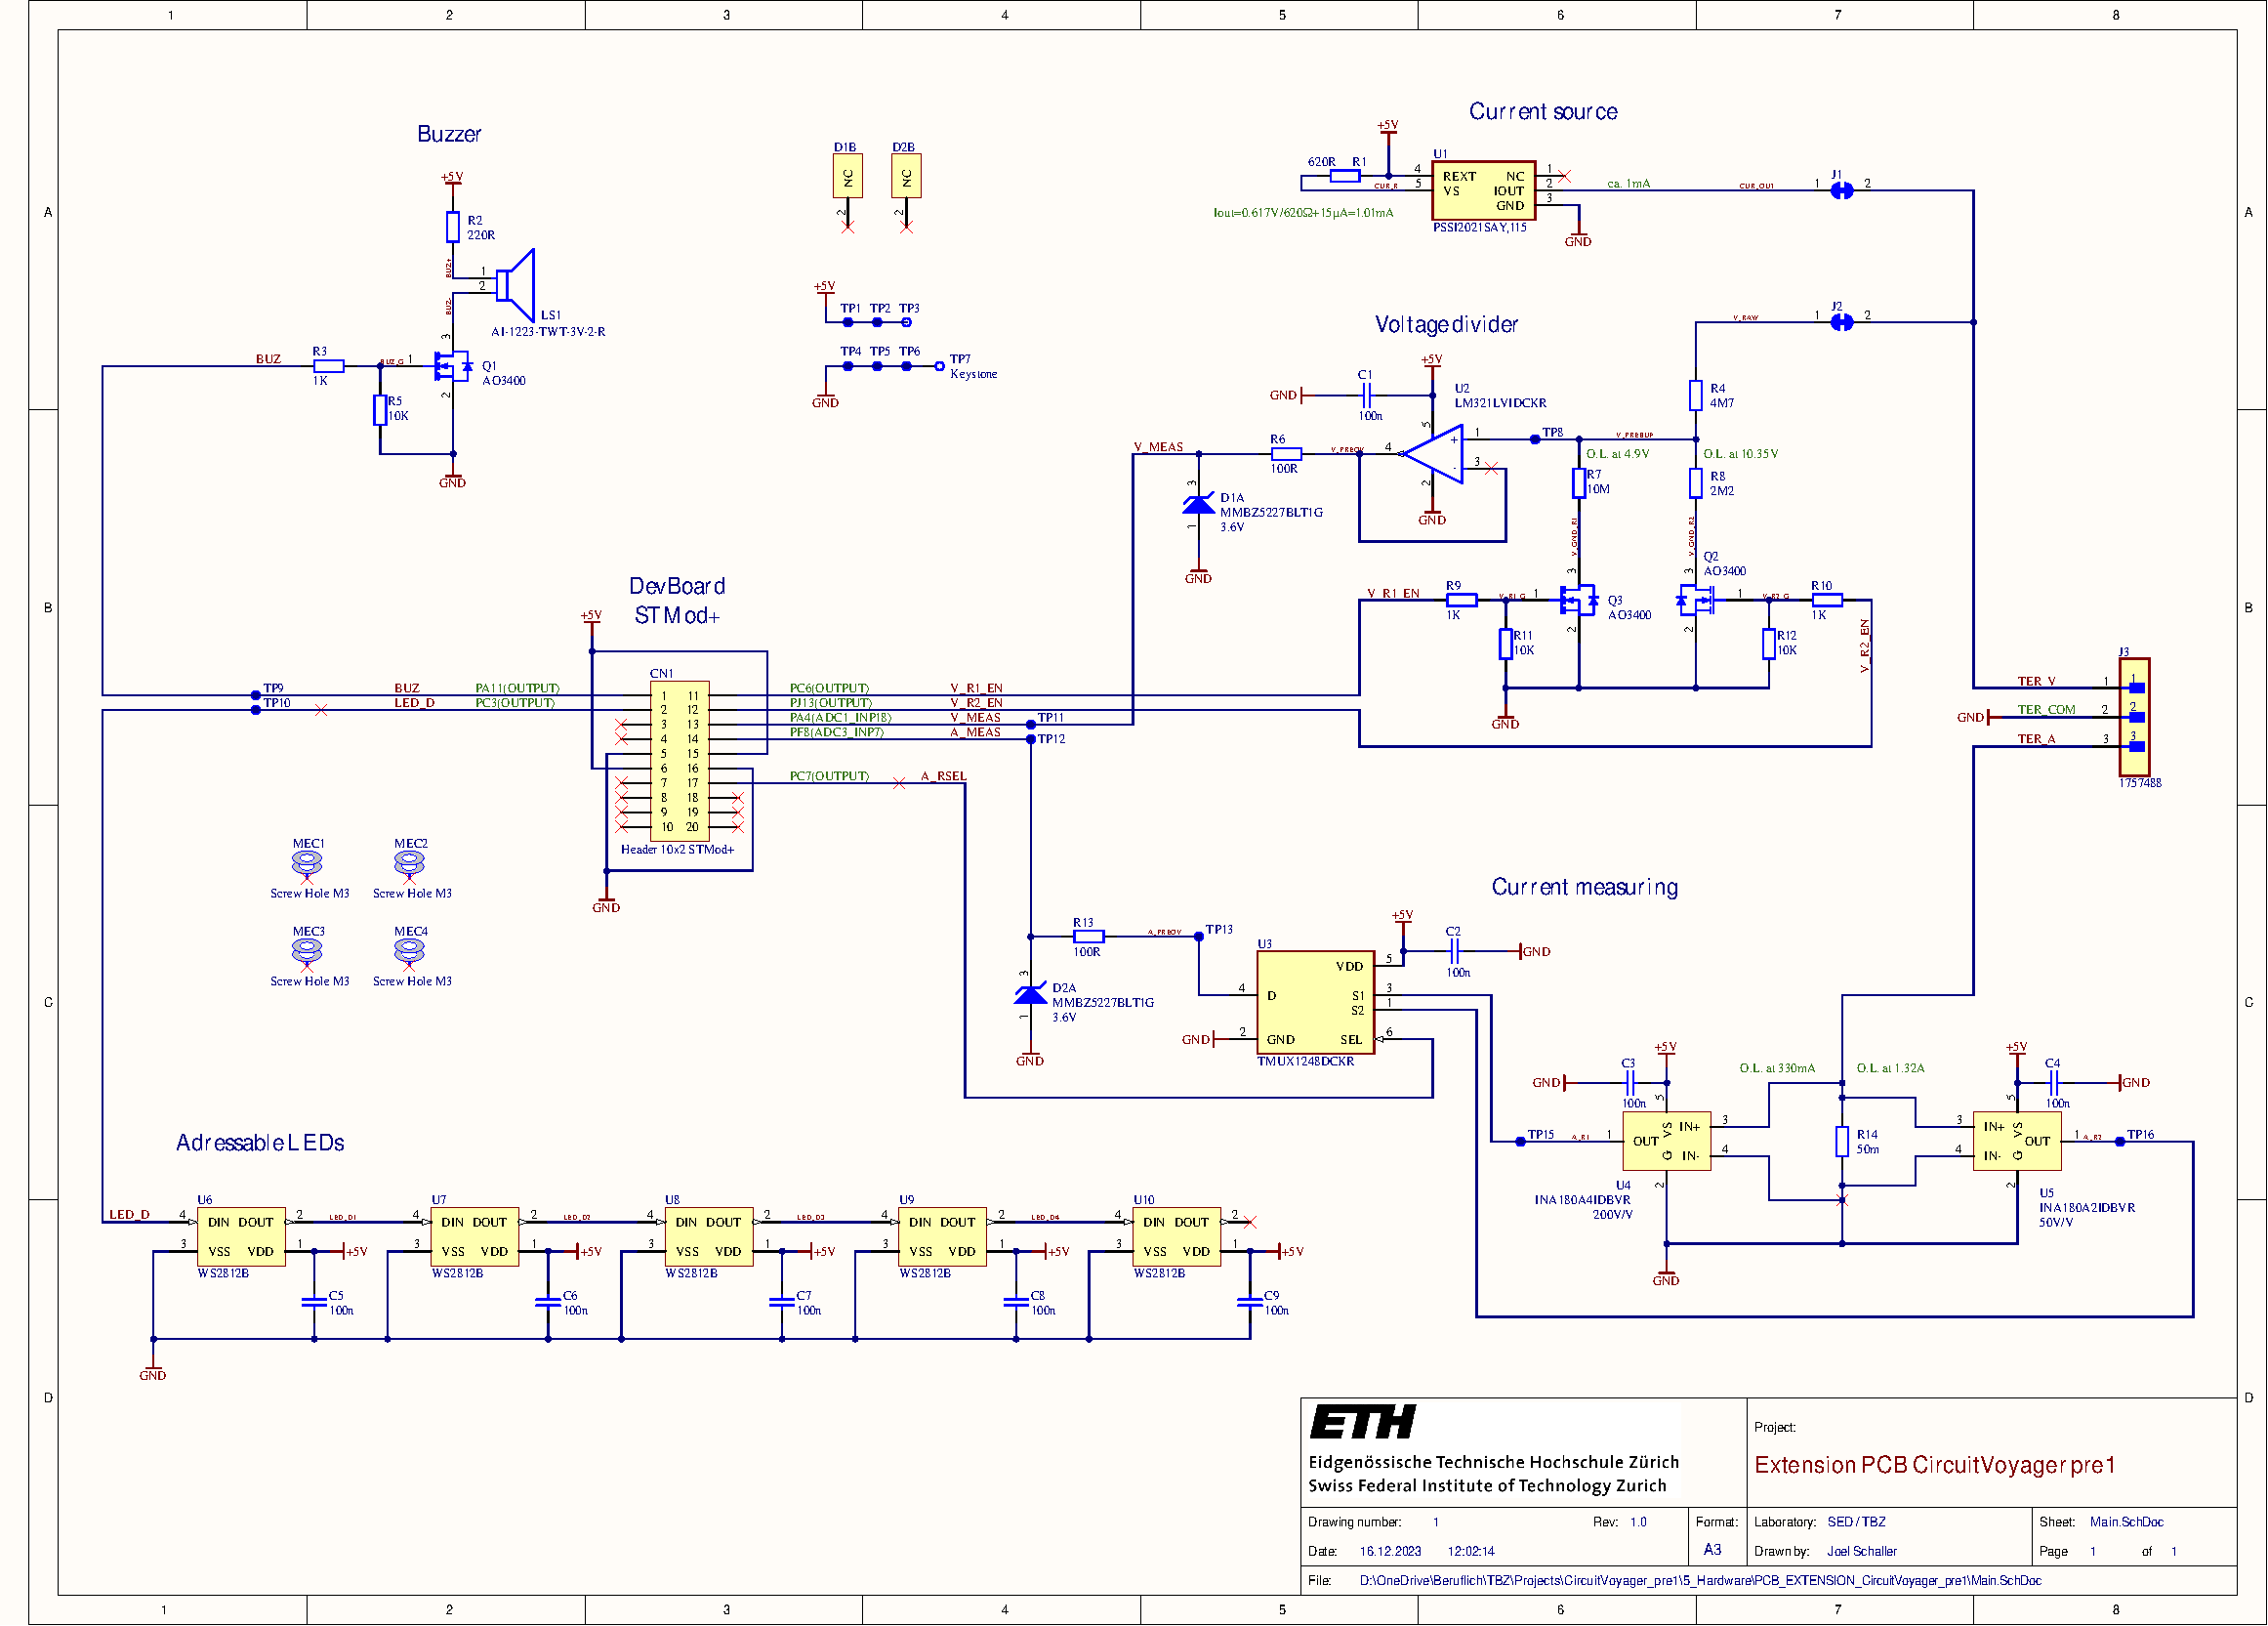
\includegraphics[width=12cm, trim={23cm 15cm 6cm 5cm}, clip]{../../../5_Hardware/PCB_EXTENSION_CircuitVoyager_pre1/Project Outputs for PCB_EXT_CV_PRE1/Schematic_PCB_EXTENSION_CircuitVoyager_pre1.pdf}
	\caption{Voltage Divider Circuit}
	\label{fig:Voltage Divider Circuit}
\end{figure}

The voltage divider is used to measure voltages over the V terminal. This circuit is one approach to range switching, which is described more detailed in the following chapter [Write more detailed text about how to execute range switching and what are the pros and cons. Minimum 3 options]. This voltage divider features 2 ranges and I came up with this idea by myself. The ranges are calculated as following:
\[U_{OL(R1)} = \frac{(R_4 + R_7) \cdot U_{OL(MCU)}}{R_7} = \frac{(4.7M\Omega + 10M\Omega) \cdot 3.3V}{10M\Omega} = \underline{\underline{4.851V}}\]
\[U_{OL(R2)} = \frac{(R_4 + R_8) \cdot U_{OL(MCU)}}{R_8} = \frac{(4.7M\Omega + 2.2M\Omega) \cdot 3.3V}{2.2M\Omega} = \underline{\underline{10.35V}}\]
This divided voltage is then fed into an impedance converter which guarantees that the voltage divider isn't manipulated by the ADC internal resistance and also helps on the DevBoards analog paths, because they're very long and therefore vulnerable to electromagnetic fields.

\textbf{
\begin{textbf}
Text to put into ranges part:
This range switching part has the advantage of using many ranges at once, as for example with 2 range switches can use 3 different ranges and with 3 range switches can use 7 ranges. On the other hand it has the disadvantage of only being able to divide the input voltage and not being able to amplify. Additionally, the internal resistance is always changing and therefore impacting the DUT. I wouldn't recommend this circuit because of said factors and only switch on the measured side. For example use different Amps / Divs to create the right voltage ranges and only switch the high Z path, that doesn't have an impact on the DUT.
\end{textbf}}




\subsubsection{Current Source Circuit}

\begin{figure}[H]
	\centering
	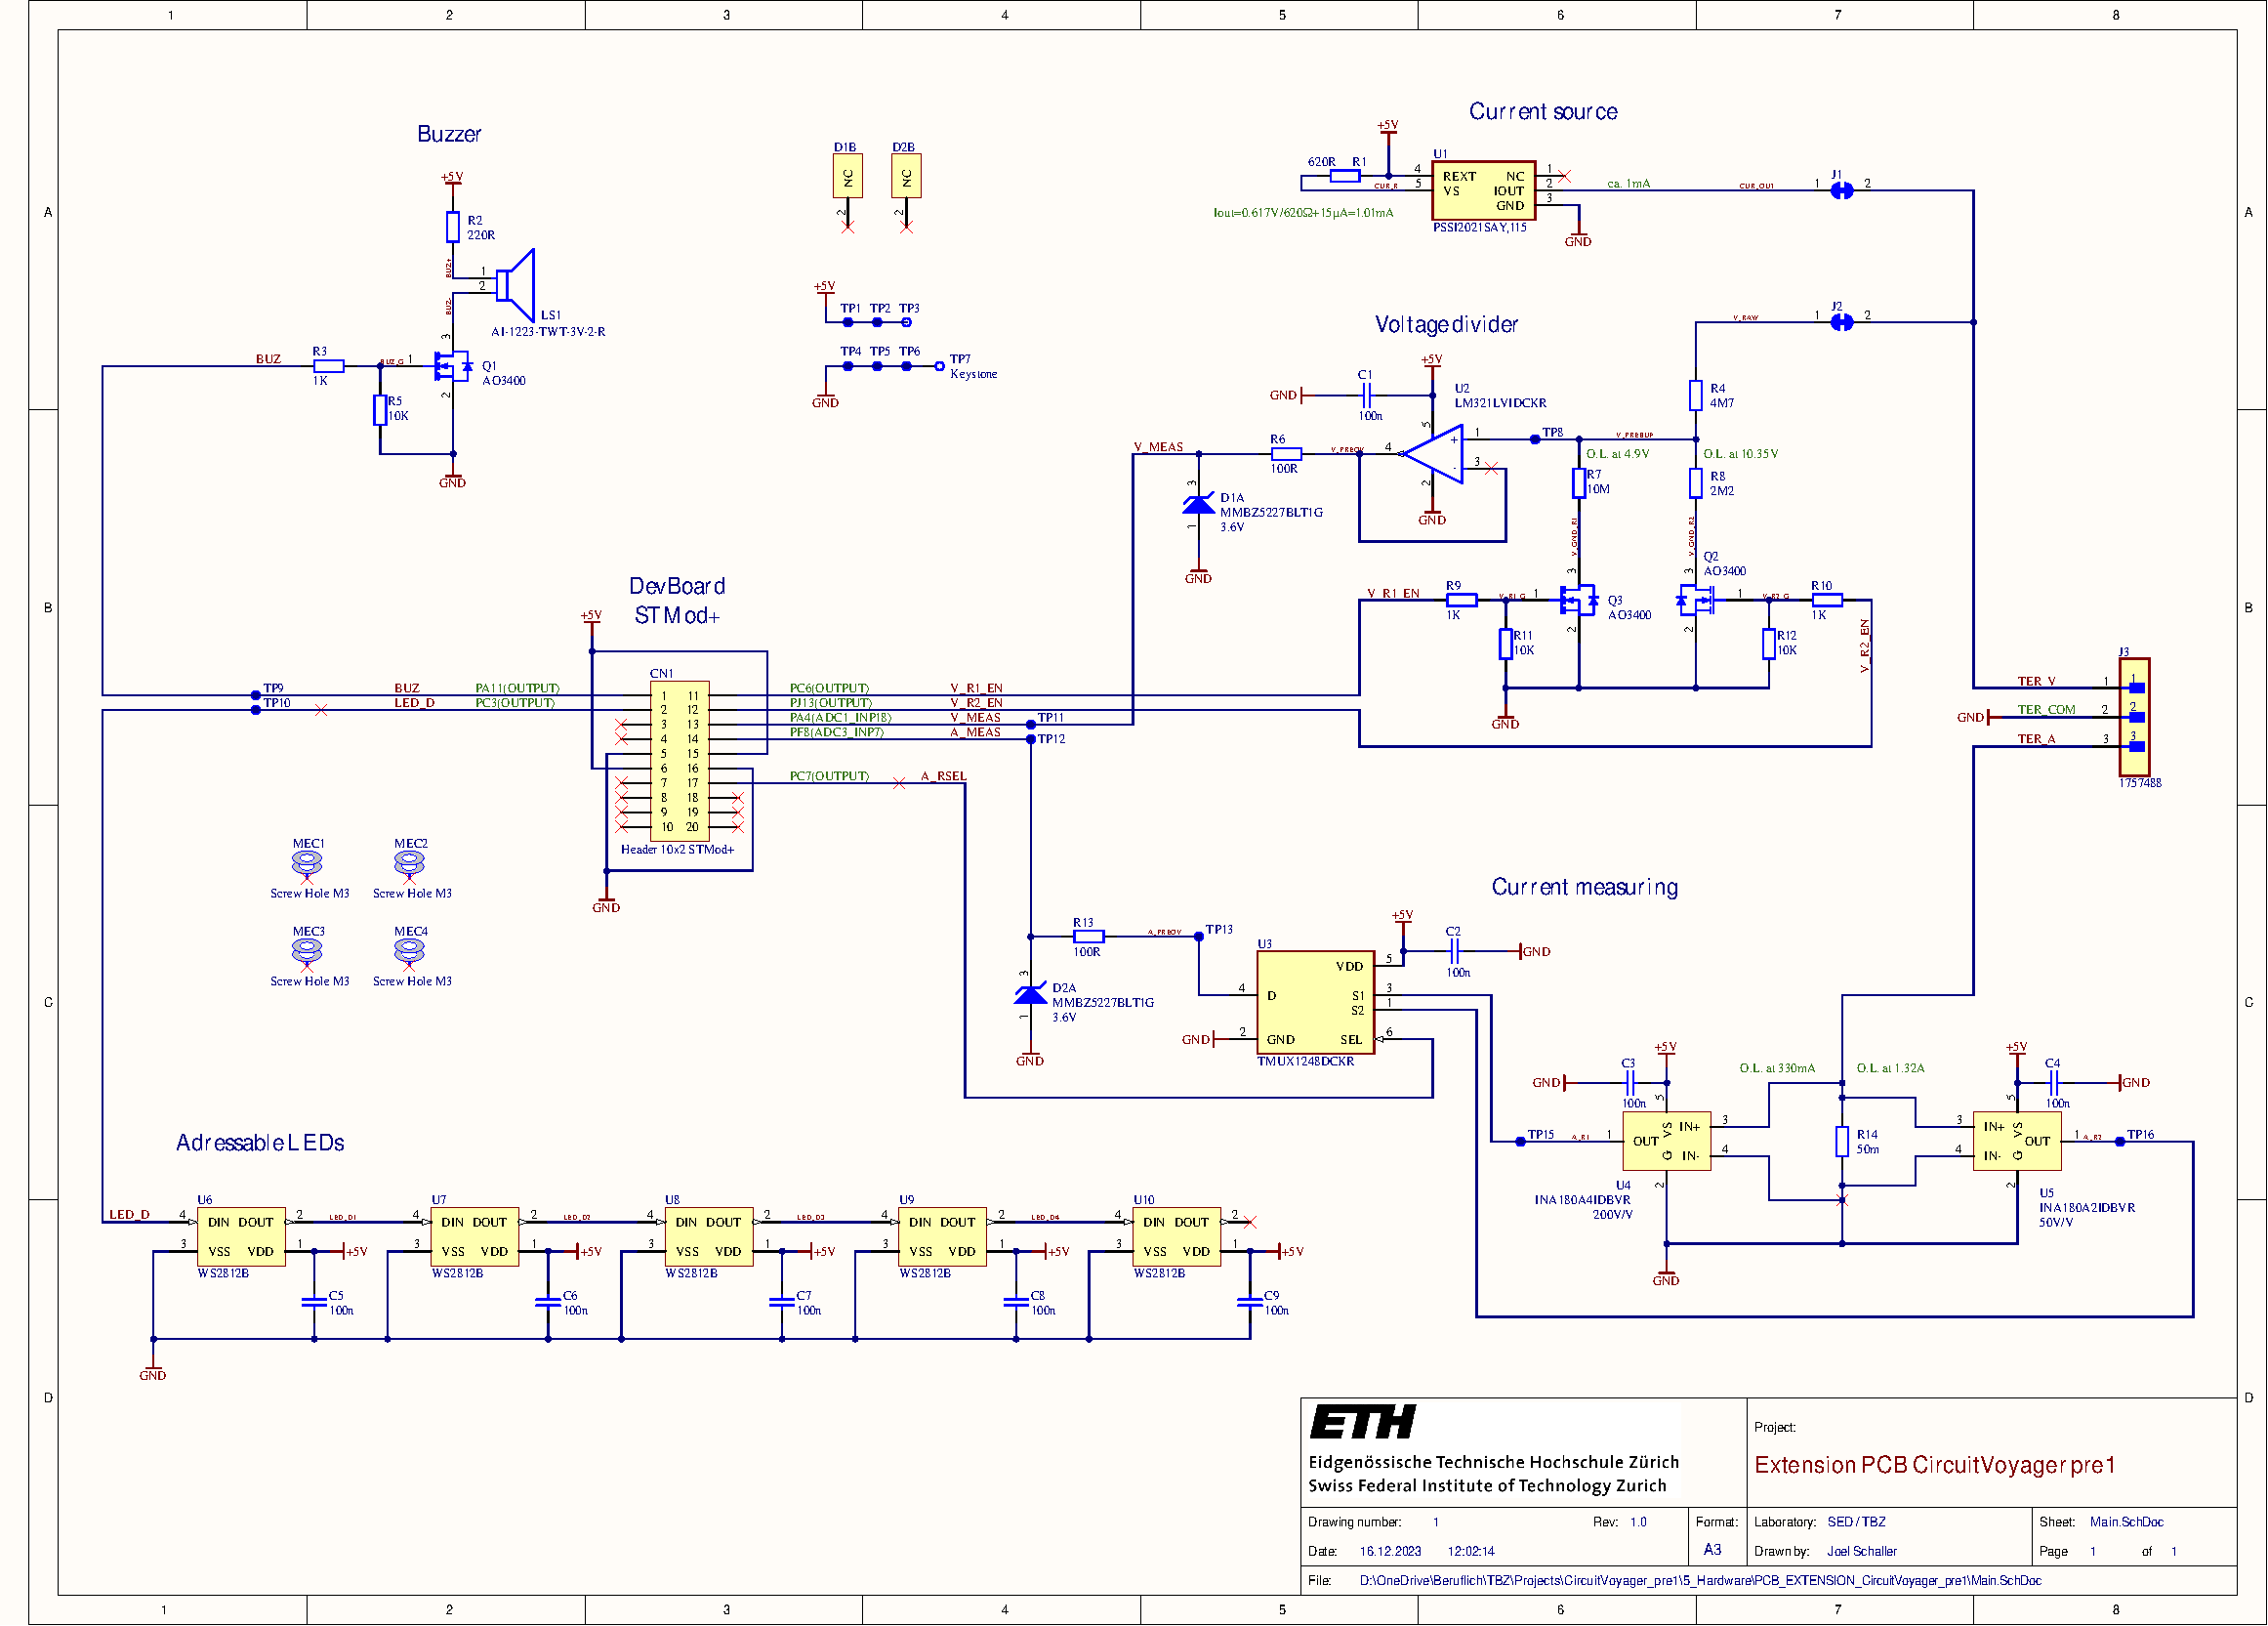
\includegraphics[width=10cm, trim={20cm 23cm 10cm 1cm}, clip]{../../../5_Hardware/PCB_EXTENSION_CircuitVoyager_pre1/Project Outputs for PCB_EXT_CV_PRE1/Schematic_PCB_EXTENSION_CircuitVoyager_pre1.pdf}
	\caption{Current Source Circuit}
	\label{fig:Current Source Circuit}
\end{figure}

The current source circuit will be used to measure continuity and resistance together with the voltage measuring function. A constant current will be induced to the DUT and because the voltage over the DUT can be measured, the resistance can be calculated. The constant current can be calculated as following:
\[I_{OUT} = \frac{U_{VS}}{R_1} + 15\mu A = \frac{0.617V}{620\Omega} + 15\mu A = \underline{\underline{1.01mA}}\]
But this doesn't matter that much, because the DMM will be calibrated using the solderbridge J1.


\subsubsection{Current Measuring Circuit}

\begin{figure}[H]
	\centering
	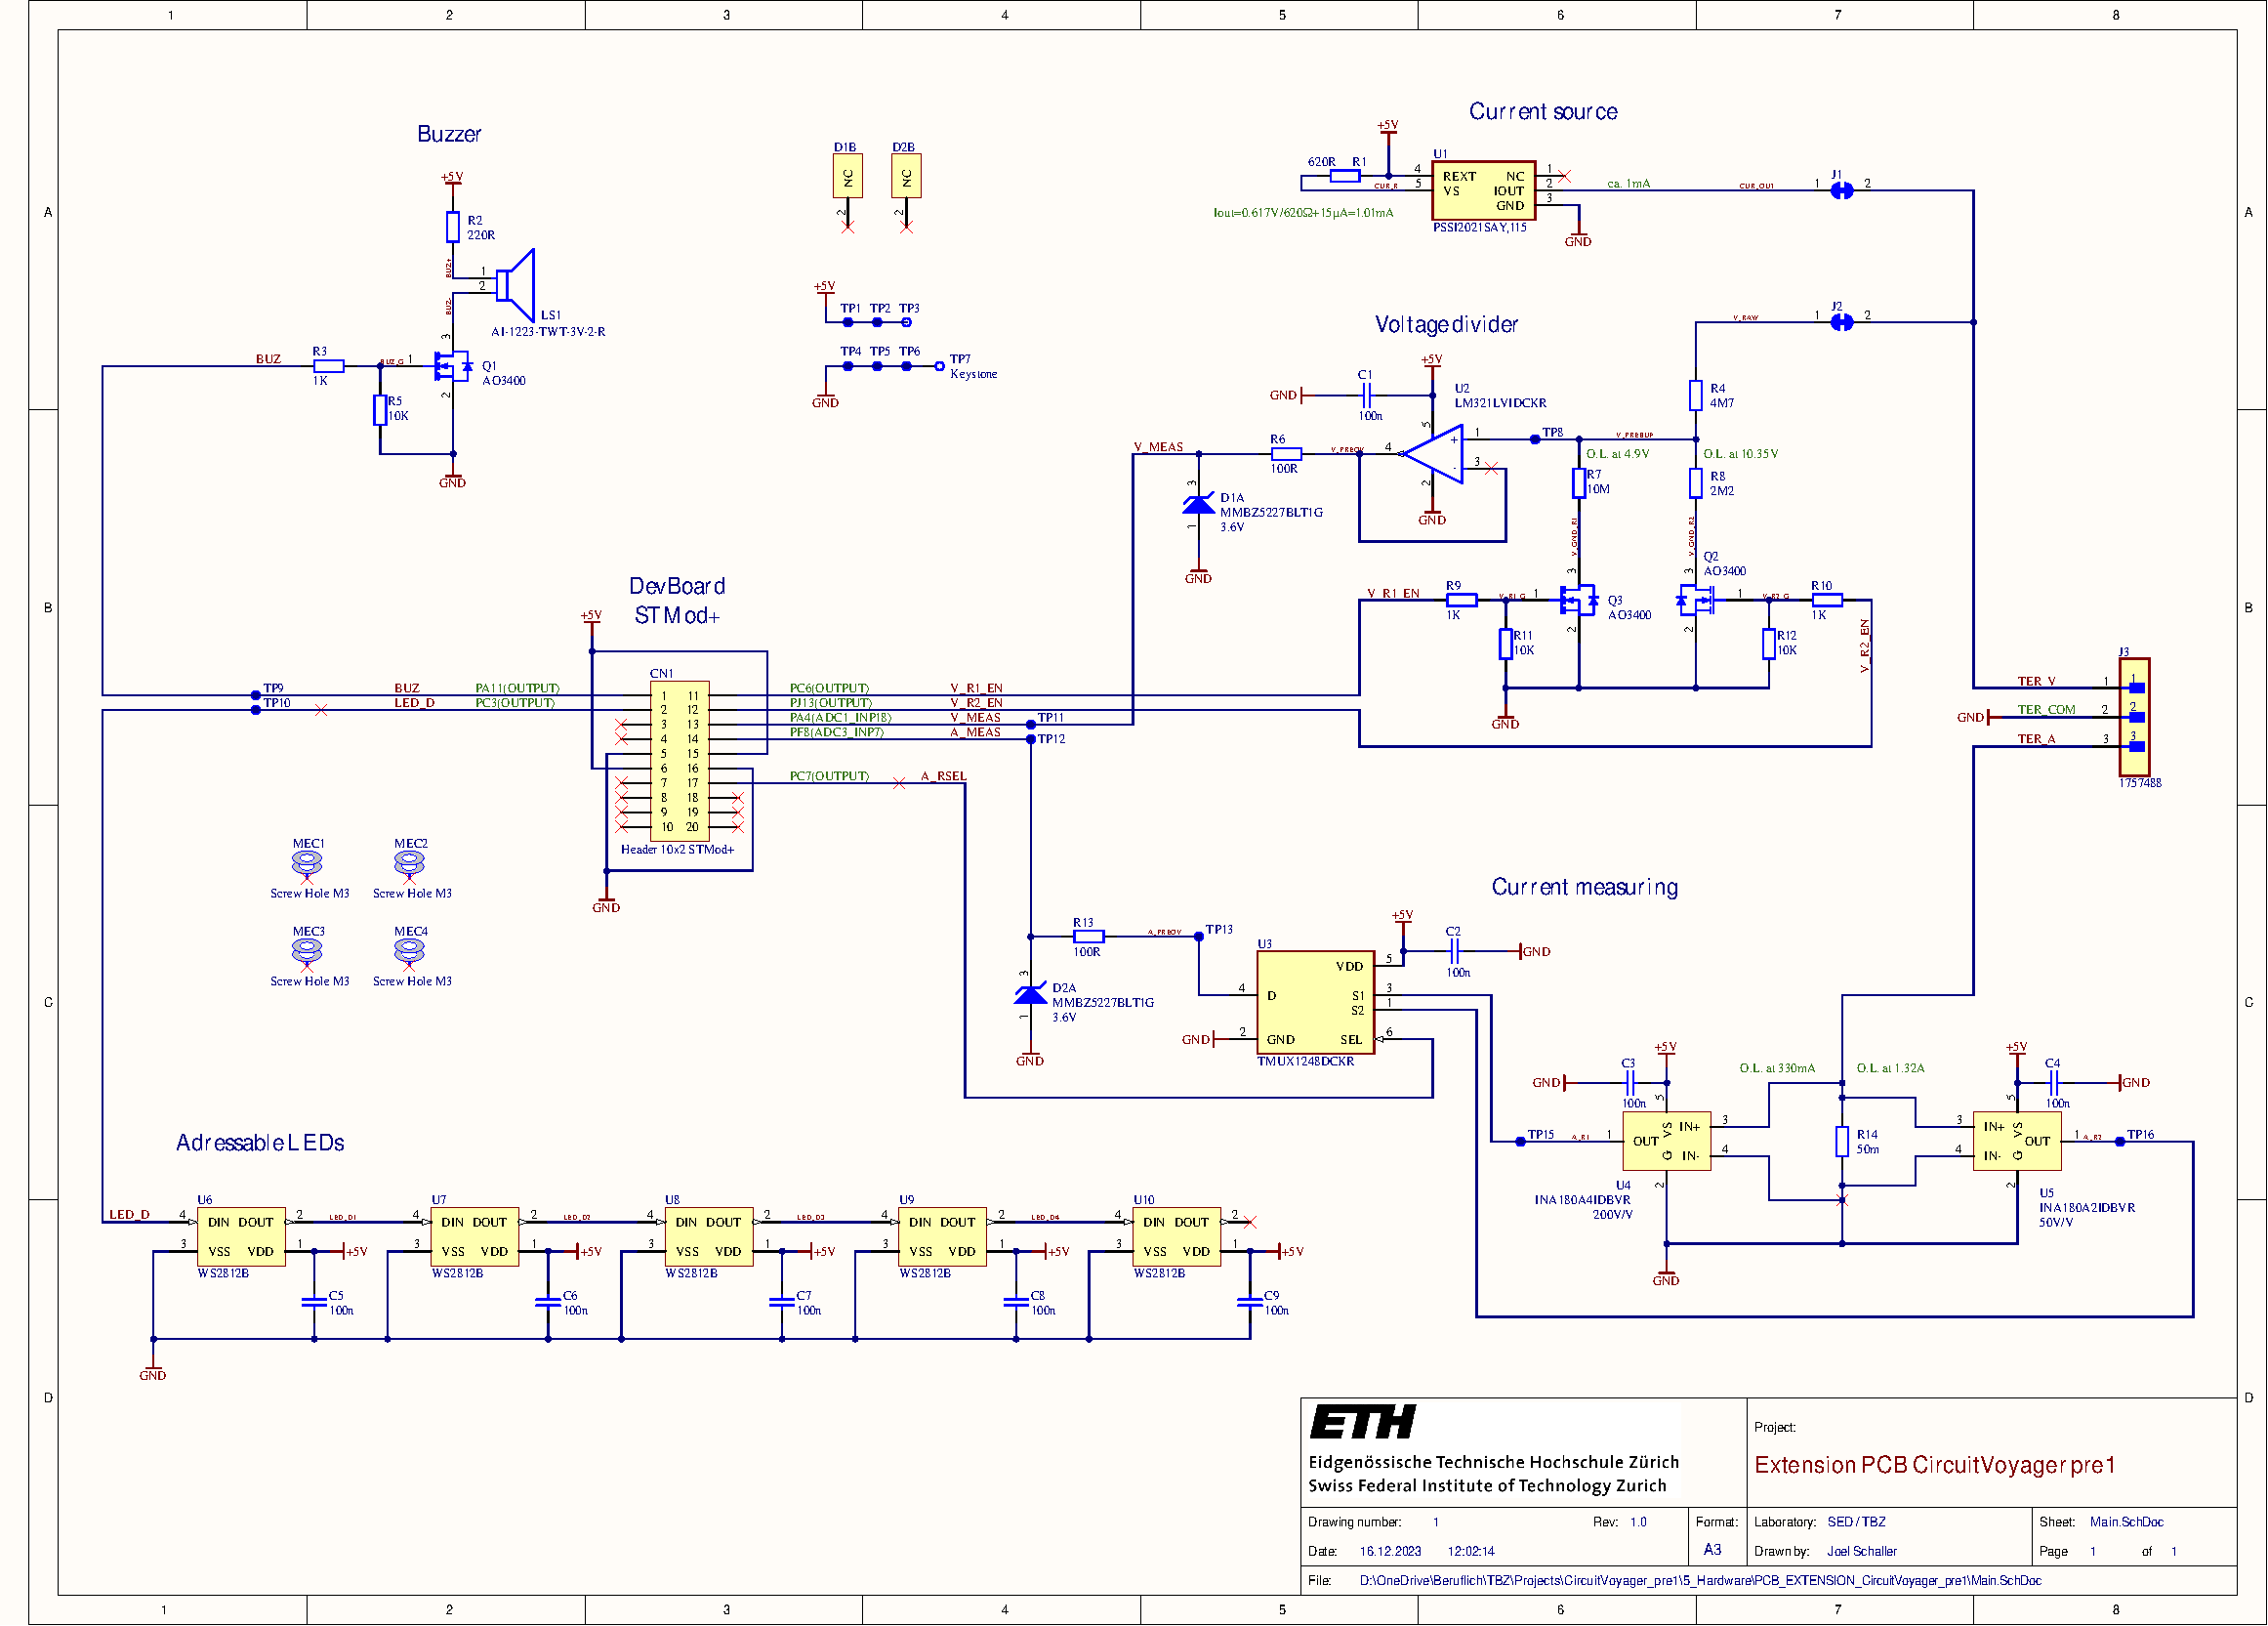
\includegraphics[width=14cm, trim={19.5cm 5cm 1cm 14.5cm}, clip]{../../../5_Hardware/PCB_EXTENSION_CircuitVoyager_pre1/Project Outputs for PCB_EXT_CV_PRE1/Schematic_PCB_EXTENSION_CircuitVoyager_pre1.pdf}
	\caption{Current Measuring Circuit}
	\label{fig:Current Measuring Circuit}
\end{figure}

The current measuring circuit is used to measure currents with the A terminal. This circuit is one approach to range switching, which is described more detailed in the following chapter [Write more detailed text about how to execute range switching and what are the pros and cons. Minimum 3 options]. This circuit features 2 ranges and I came up with this idea, while reading some articles on DMMs \cite{Digital_multimeter_circuit_using_ICL7107} \cite{AN-202_A_Digital_Multimeter_Using_the_ADD3501}. The ranges are calculated as following:
\[I_{OL(R1)} = \frac{U_{OL(MCU)}}{R_{14} \cdot G_{U4}} = \frac{3.3V}{50m\Omega \cdot 200\frac{V}{V}} = \underline{\underline{330mA}}\]
\[I_{OL(R2)} = \frac{U_{OL(MCU)}}{R_{14} \cdot G_{U5}} = \frac{3.3V}{50m\Omega \cdot 50\frac{V}{V}} = \underline{\underline{1.32A}}\]
These voltages are then fed into an analog MUX, which switches the processed voltages to the ADC. This has the advantage, that the DMM doesn't manipulate the actual path, where the current is flowing through and therefore not influencing the DUT.

The power rating of R14 is 125mW, while the maximal power loss of R14 at 1.32A is 87.12mW.
\[P_{R14} = I^2 \cdot R = (1.32A)^2 \cdot 50m \Omega = \underline{\underline{87.12mW}}\]



\newpage
\subsection{PCB}
\subsubsection{Layout}

The PCB layout was also made in Altium Designer. This was therefore also my first layout in Altium Designer. The only problem I had, were the vias and imporvised them by setting their parameters manually. 

\begin{figure}[H]
	\centering
	\includegraphics[width=5.5cm, page=2]{Resources/PCB_LAyout.png}
	\caption{Extension PCB Layout}
	\label{fig:Extension PCB Layout}
\end{figure}

Later I've generated the output files (Gerber files, BOM, assembly drawing) and ordered the PCB on JLCPCB with 2 layers, tented vias, removed order number and blue solder mask. The BOM is in the appendix chapter: \ref{sec:Extension PCB Manufacture 11.23 BOM}. The components were sourced using DigiKey and ETH SPH.

\subsubsection{Assembly}

Then I've assembled the PCB by hand, which wasn't a problem at all. But it turned out, that I've ordered the wrong connectors for the STMod interface. Instead of the 4 mm long pins I've ordered the 2 mm long pins, which don't make contact with the socket from the DevBoard. But luckily I was able to order longer ones, which arrived quite fast.

\begin{figure}[H]
	\centering
	\includegraphics[height=10cm, page=2]{../../../5_Hardware/PCB_EXTENSION_CircuitVoyager_pre1/Project Outputs for PCB_EXT_CV_PRE1/PCB_EXTENSION_CircuitVoyager_pre1.pdf}
	\caption{Extension PCB Assembly Drawing}
	\label{fig:Extension PCB Assembly Drawing}
\end{figure}



\begin{figure}[H]
	\centering
	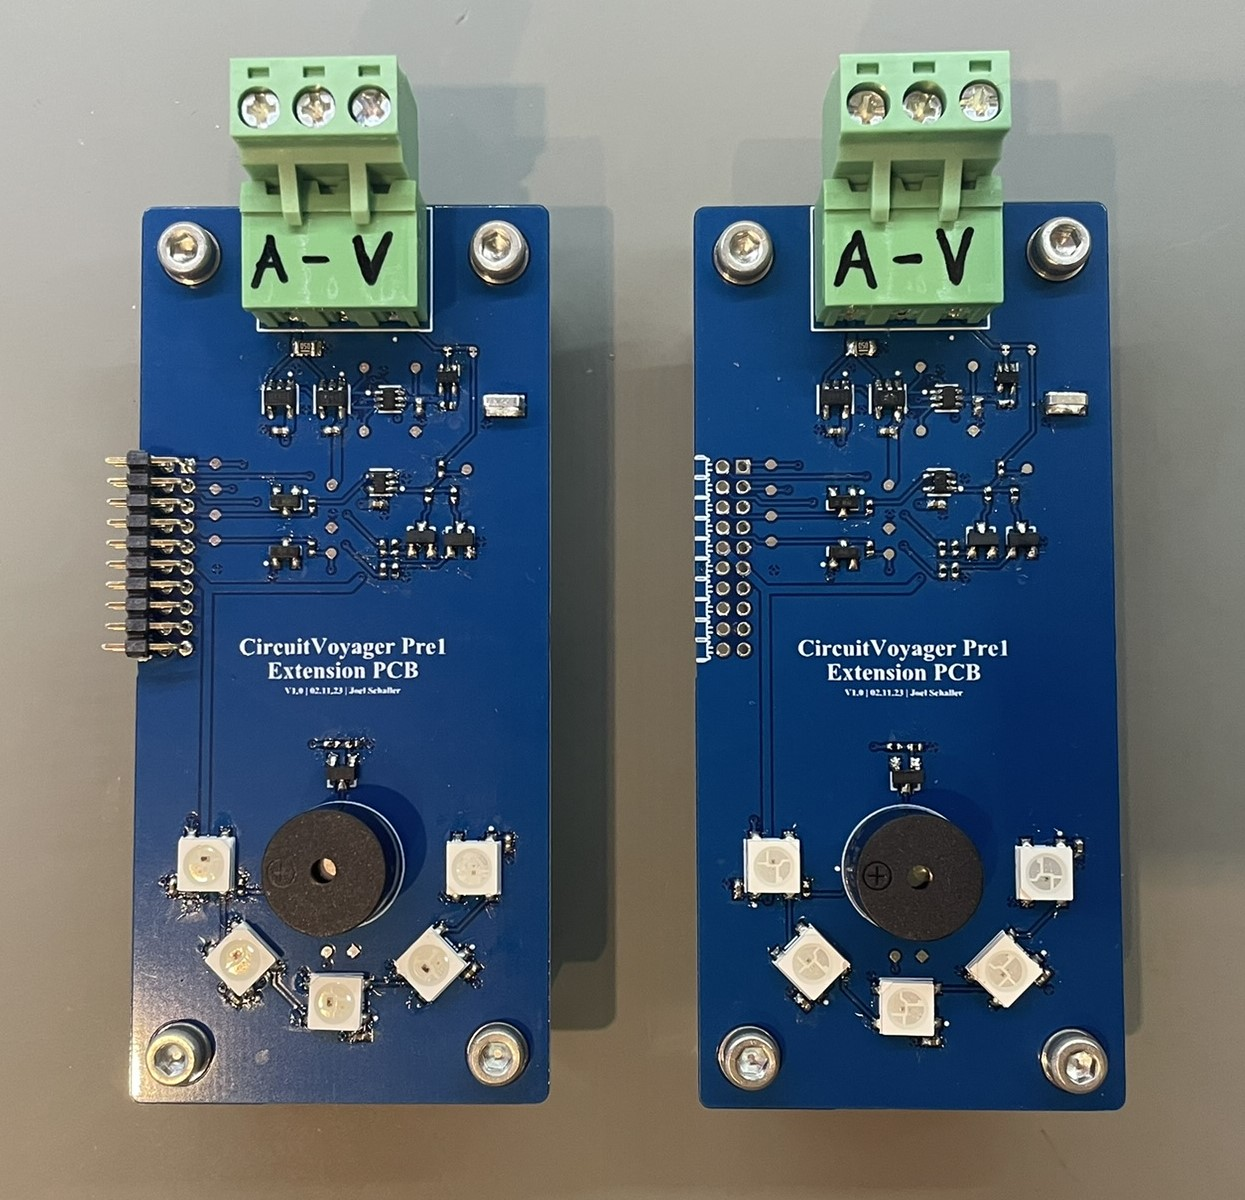
\includegraphics[height=8cm]{Resources/PCB.png}
	\caption{Extension PCB}
	\label{fig:Extension PCB}
\end{figure}

\newpage
\subsubsection{Commissioning}
I've only documented one commission of the 2 PCBs. The other one was tested with the same process.

\begin{table}[H]
	\centering
	\label{tab:commissioning PCB 1}
\begin{tabular}{|| c | c | c | c ||} 
\hline
Action & Measurement point & Expected & Measured \\ [0.5ex] 
\hline\hline
Connect power supply @ 5V & CN1.6 \(\rightarrow\) TP7 & max. 100mA & \textcolor{Green}{\textbf{18mA}} \\
\hline
Test Buzzer (TP9 to 3.3V) & acoustic & beeps & \textcolor{Green}{\textbf{PASS}} \\
\hline
Test const. Current & J3.1 & 1mA & \textcolor{Red}{\textbf{13mA}} \\
\hline
LEDs on with AWG (CN1.2) & optical & lights up & \textcolor{Green}{\textbf{PASS}} \\
\hline
Current meas. test Range 1 & CN1.14 & 10V/A & \textcolor{Green}{\textbf{fig: \ref{fig:Commissioning PCB1 current measurements}}} \\
\hline
Current meas. test Range 2 & CN1.14 & 2.5V/A & \textcolor{Green}{\textbf{fig: \ref{fig:Commissioning PCB1 current measurements}}} \\
\hline
Voltage meas. test Range 1 & CN1.13 & 0.68V/V & \textcolor{Green}{\textbf{fig: \ref{fig:Commissioning PCB1 voltage measurements}}} \\
\hline
Voltage meas. test Range 2 & CN1.13 & 0.32V/V & \textcolor{Green}{\textbf{fig: \ref{fig:Commissioning PCB1 voltage measurements}}} \\
\hline
\end{tabular}
	\caption{commissioning PCB 1}
\end{table}



\begin{figure}[H]
	\centering
	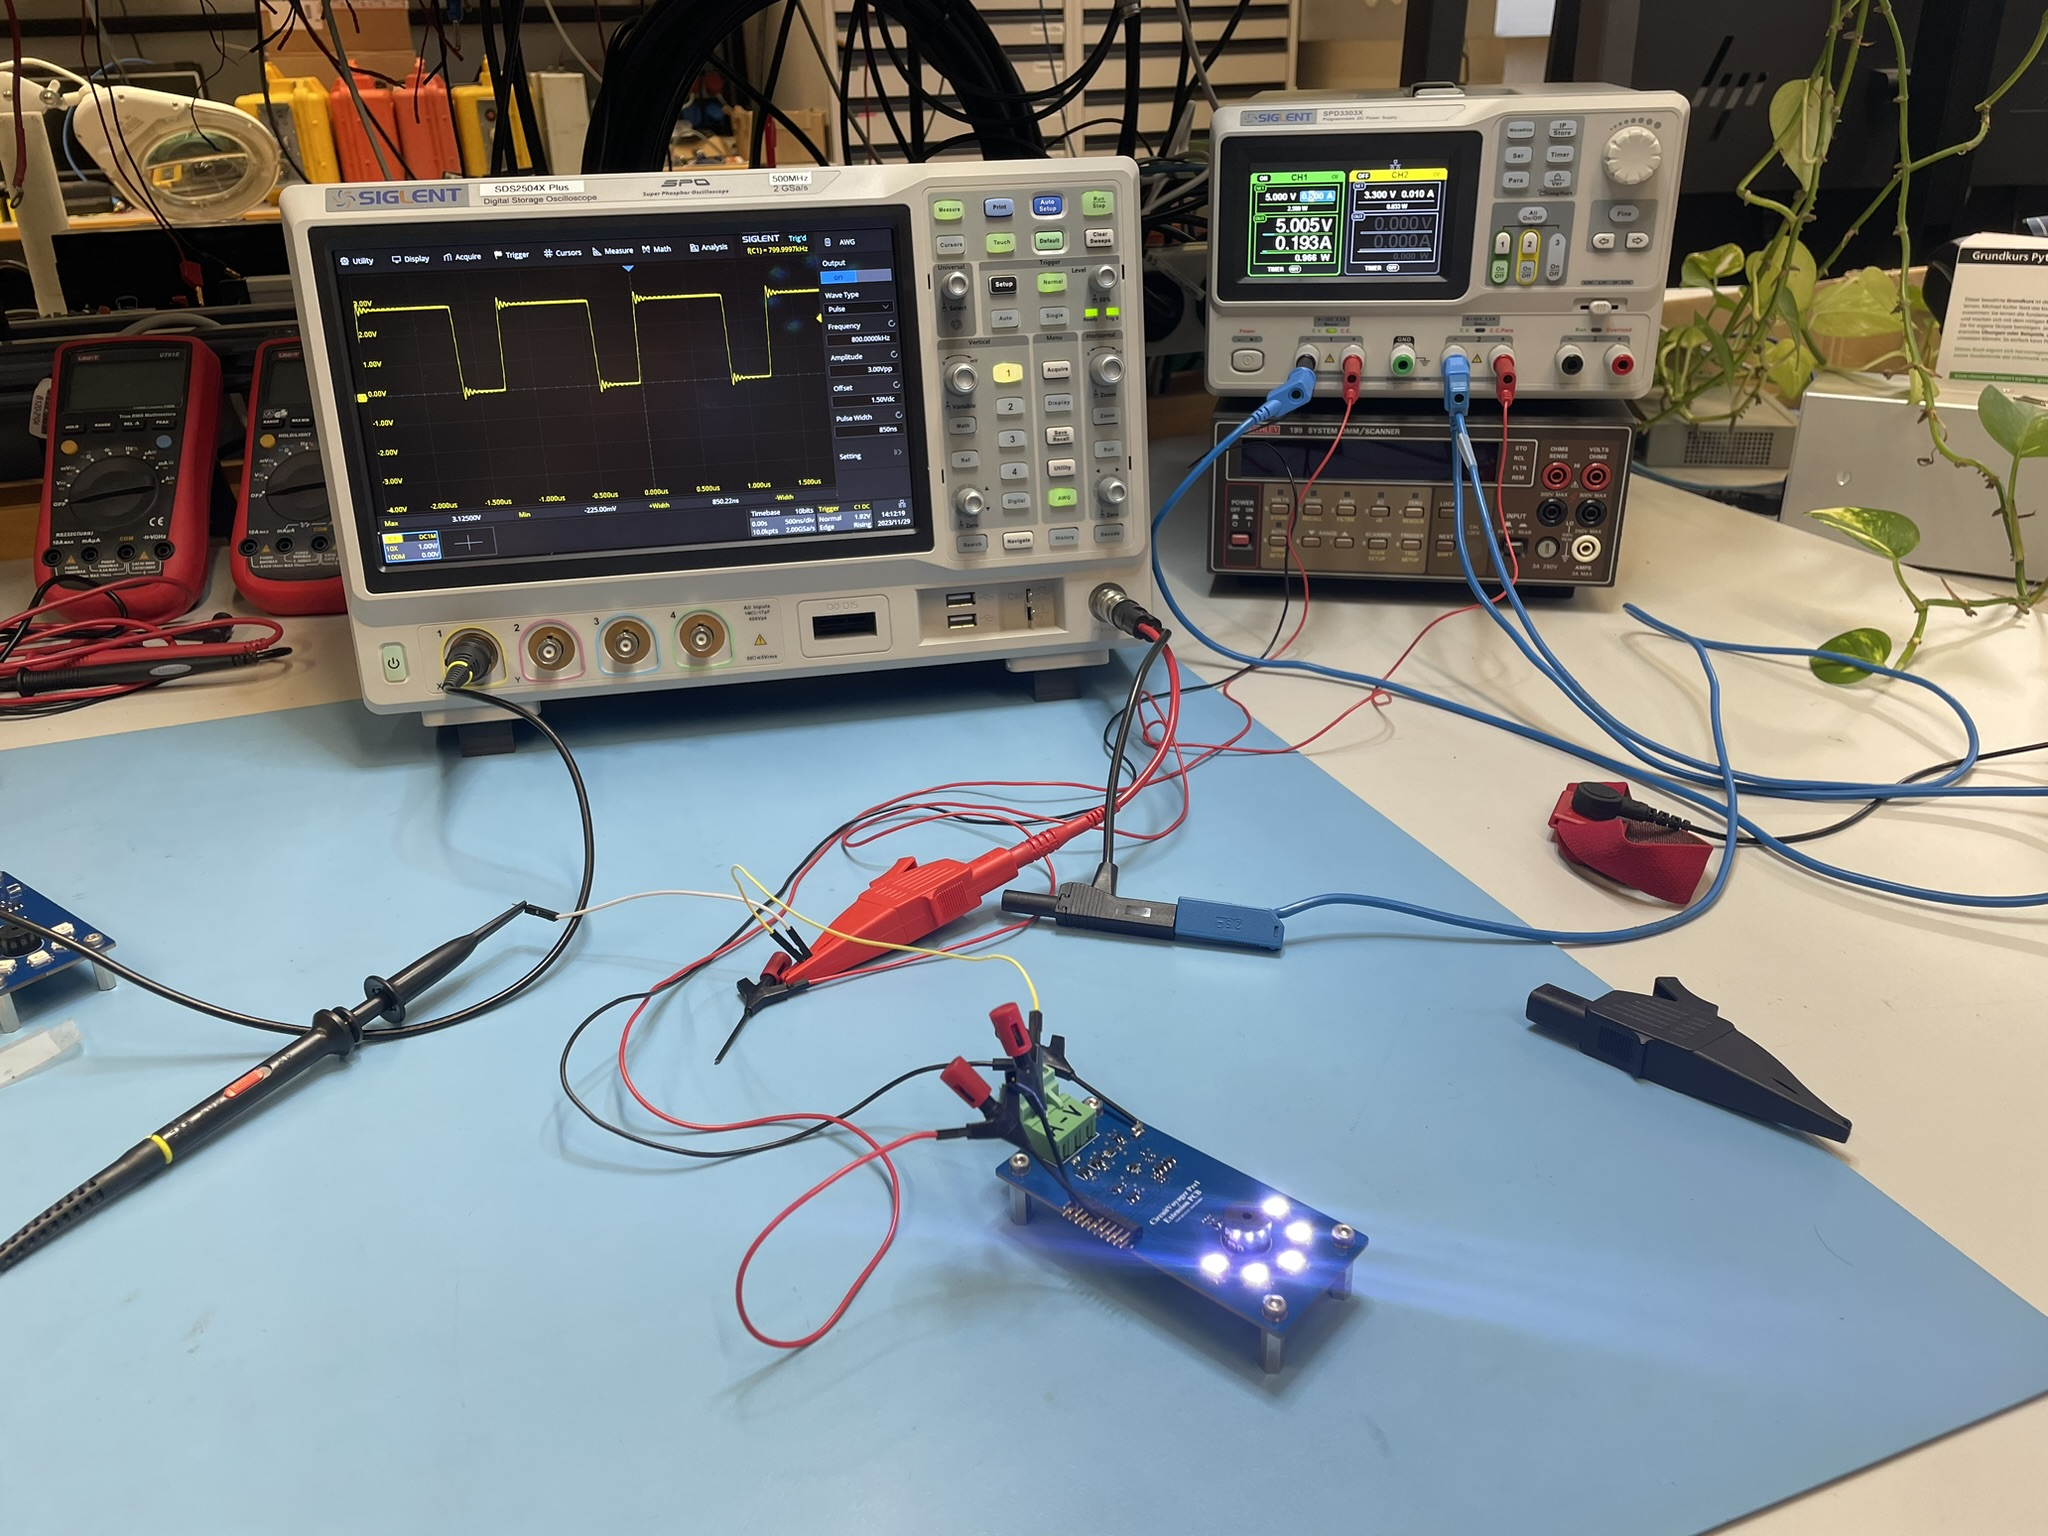
\includegraphics[width=15cm]{Resources/comissioning_lab_build.JPEG}
	\caption{Commissioning Lab}
	\label{fig:Commissioning Lab}
\end{figure}



\begin{figure}[H]
	\centering
	\begin{tikzpicture}
		\begin{groupplot}[
		group style={
			group size=1 by 2,
			horizontal sep=0cm,
			ylabels at=edge left,
		},
		width=13cm,
		height=3.5cm,
		scale only axis,
		xmin=0,xmax=1600,
		xtick distance=200,
		enlargelimits=false,
		grid=major,
		]
		
		\nextgroupplot[ylabel=$ U_{TP12(R1)} $, y unit=mV, xticklabels={}, ymin=0, ymax=3500, ytick distance=500]
		\addplot[red] coordinates { (1, 23) (5, 64) (10, 116) (50, 533) (100, 1050) (200, 2070) (400, 3320) (600, 3460) (800, 3480)};

		\nextgroupplot[ylabel=$ U_{TP12(R2)} $, y unit=mV, xlabel=$ I $,x unit=mA, ymin=0, ymax=3500, ytick distance=500]
		\addplot[ForestGreen] coordinates { (1, 7) (100, 273) (200, 544) (400, 1080) (600, 1620) (800, 2140) (1000, 2600) (1200, 2970) (1400, 3240) (1600, 3460)};
		
		\end{groupplot}
	\end{tikzpicture}
\caption{Commissioning PCB1 current measurements}
\label{fig:Commissioning PCB1 current measurements}
\end{figure}








\begin{figure}[H]
	\centering
	\begin{tikzpicture}
		\begin{groupplot}[
		group style={
			group size=1 by 2,
			horizontal sep=0cm,
			ylabels at=edge left,
		},
		width=13cm,
		height=3.5cm,
		scale only axis,
		xmin=0,xmax=16,
		xtick distance=2,
		enlargelimits=false,
		grid=major,
		]
		
		\nextgroupplot[ylabel=$ U_{TP11(R1)} $, y unit=mV, xticklabels={}, ymin=0, ymax=3500, ytick distance=500]
		\addplot[red] coordinates { (0, 0) (1, 680) (2, 1360) (3, 2020) (4, 2570) (5, 2970) (6, 3230) (7, 3400) (8, 3400)  (9, 3400)};

		\nextgroupplot[ylabel=$ U_{TP11(R2)} $, y unit=mV, xlabel=$ U $,x unit=V, ymin=0, ymax=3500, ytick distance=500]
		\addplot[ForestGreen] coordinates { (0, 0) (1, 320) (2, 640) (3, 950) (4, 1270) (5, 1590) (6, 1890) (7, 2180) (8, 2450) (9, 2670) (10, 2860) (11, 3010) (12, 3140) (13, 3250) (14, 3340) (15, 3400) (16, 3400) };
		
		\end{groupplot}
	\end{tikzpicture}
\caption{Commissioning PCB1 voltage measurements}
\label{fig:Commissioning PCB1 voltage measurements}
\end{figure}


%\textit{FUCKING RAIL TO RAIL OP NEH...}

%\textit{text über abflachung in grafix wegen zdiode.}

\newpage

\subsubsection{Bad Design}
During the commissioning I noticed, that some of my circuit are kind of misconstructions. This is due to my missing design review but gives me the opportunity to reflect a lot and learn about my fault the hard way.

So first my Current Source has the problem, that is directly connected to the V terminal which is done correct, only considering the resistance mode of the DMM. But when trying to measure a voltage, the current source will inject a current into the voltage measuring circuit which makes the voltage measuring circuit / mode unusable. So the current source should be able to be turned off, to use the voltage mode of the DMM. Because I don't have enough time to fix this problem, I will cut through J1.

The current source also doesn't work as intended, as the const. current which should be 1mA is now around 13mA. But I don't bother, cause I won't use the current source anyways.

See also: Figure \ref{fig:Extension PCB Schematics}







\newpage
\section{The MCU}
For this project I've chosen a high speed microcontroller. I'm using an STM32H747-XIH6U. The special thing about this MCU is, that it has 2 cores. The main core is a Cortex M7 at a frequency of up to 480MHz and the second one is a Cortex M4 running at up to 240MHz. But this also means that it's a bit expensive at about 20 CHF. This MCU also features 1 MB of flash per core and a total of 1 MB of RAM. But these memories can get full rather quickly, when working with graphical displays or the USB stack for example. That's why I'm using an external flash and RAM in this project.


\section{STM32 Multicore Debugging}
As usual, I'll be testing the DevBoard by programming a good old blink sketch. The information for this multicore blink sketch I got from Controller Tech's YouTube channel \cite{YT_CT_Mutlicore_Debugging}, because the official SW documentation from STM isn't that good, and therefore I wasn't able to get the information I needed to run my first sketch.

\subsection{Procedure}
\begin{enumerate}
	\item Create a project with the STM32 Cube template for the STM32H747XIH6. (Using default configuration)
	\item Set up the RCC to use the external oscillator and configure clocks to their maximum frequencies.
	\item Set up the GPIOs of for the debug LEDs. Special is, that you have to assign a core to each GPIO pin. This parameter says, which core is able to manipulate said GPIO and in which under project (CM4 or CM7) has the define with the GPIO name defined. 
		\begin{table}[H]
			\centering
			\label{tab:LED Annotation}
		\begin{tabular}{|| c | c | c | c | c ||} 
		\hline
		STM32 pin & LED number & LED color & Name in code & Core \\ [0.5ex] 
		\hline\hline
		PI12 & LED1 & Green & LED\_G & CM7 \\
		\hline
		PI13 & LED2 & Orange & LED\_O & CM7 \\
		\hline
		PI14 & LED3 & Red & LED\_R & CM4 \\
		\hline
		PI15 & LED4 & Blue & LED\_B & CM4 \\
		\hline
		\end{tabular}
			\caption{LED Annotation}
		\end{table}
	\item Under: Project Manager \(\rightarrow\) Code Generator: Enable the option: "Generate Peripheral initialization as a pair of .c/.h files per peripheral".
	\\ This should make the project more structurized.
	\item Generate code.
	\item Now 2 under projects are created, for each core one. Rather than using the standard files, that are already full of redundant information, I will create my own main files, with the advantage that they're also easily separable between the CM4 and CM7. The files written by me are stored in the folders "Core/Usercode"
	\item Write the code to blink the LEDs for each core:
		\lstset{language=C,caption={Blink Code CM4},label=DescriptiveLabel, style=mystyle}
		\begin{codeblock}
			\lstinputlisting{../../../6_Software/blink dual core/CM4/Core/Usercode/usermain_CM4.c}
		\end{codeblock}
	\item Now configure the debug configuration for the CM7: Enable "Halt all cores" and under Startup add the CM4 config with the "Debug" Build configuration selected.
	\item Now configure the debug configuration for the CM4: set port to 61237, set reset behaviour type to "None" and under Startup \(\rightarrow\) Edit: uncheck the download option.
	\item Now to flash the MCU it's important, that all files are saved, because they're not saved automatically as usually in single core projects. Then Click on the "Run" button, with the CM7 configuration selected, the CM4 won't work.
	\item To debug the MCU also save all files and then start debugging with the CM7 configuration selected. After the CM7 session started, click again on the debug button and start the session for the CM4. Now run both threads simultaneously by selecting them both with the "Ctrl" key and then starting them. After those threads started and the clock is configured, they can be manipulated separately.
\end{enumerate} 

Additionally, I'd recommend watching the video from Controllers Tech, as it's really informative. \cite{YT_CT_Mutlicore_Debugging} For Example Controllers Tech explains how the startup of the cores work and how you can disable cores. There are also more videos from Controllers Tech in this "Multi Core STM32" series.



\section{Boot Problems}
While programming the MCU for the first times, I had the problem that the MCU wasn't detected sometimes by the ST-Link. Therefore, the MCU wasn't resetable nor new firmware could be uploaded. It turned out, that the ST-Link could program the MCU again, when accessing the BOOT mode, which is intended to boot the MCU over USB DFU. But this mode also stops the MCU from starting the script and therefore the ST-Link detects the MCU. The boot mode can be accessed by shorting the pads of R192. Then the MCUs memory can be erased and after removing the solderbridge, the MCU operates again as normal. After this problem, with the not detectable MCU occurred multiple times, I decided to add a button to access the boot mode. So I don't have to have a soldering iron around, when the MCU ain't detectable. This modification looks as following:

\begin{figure}[H]
	\centering
	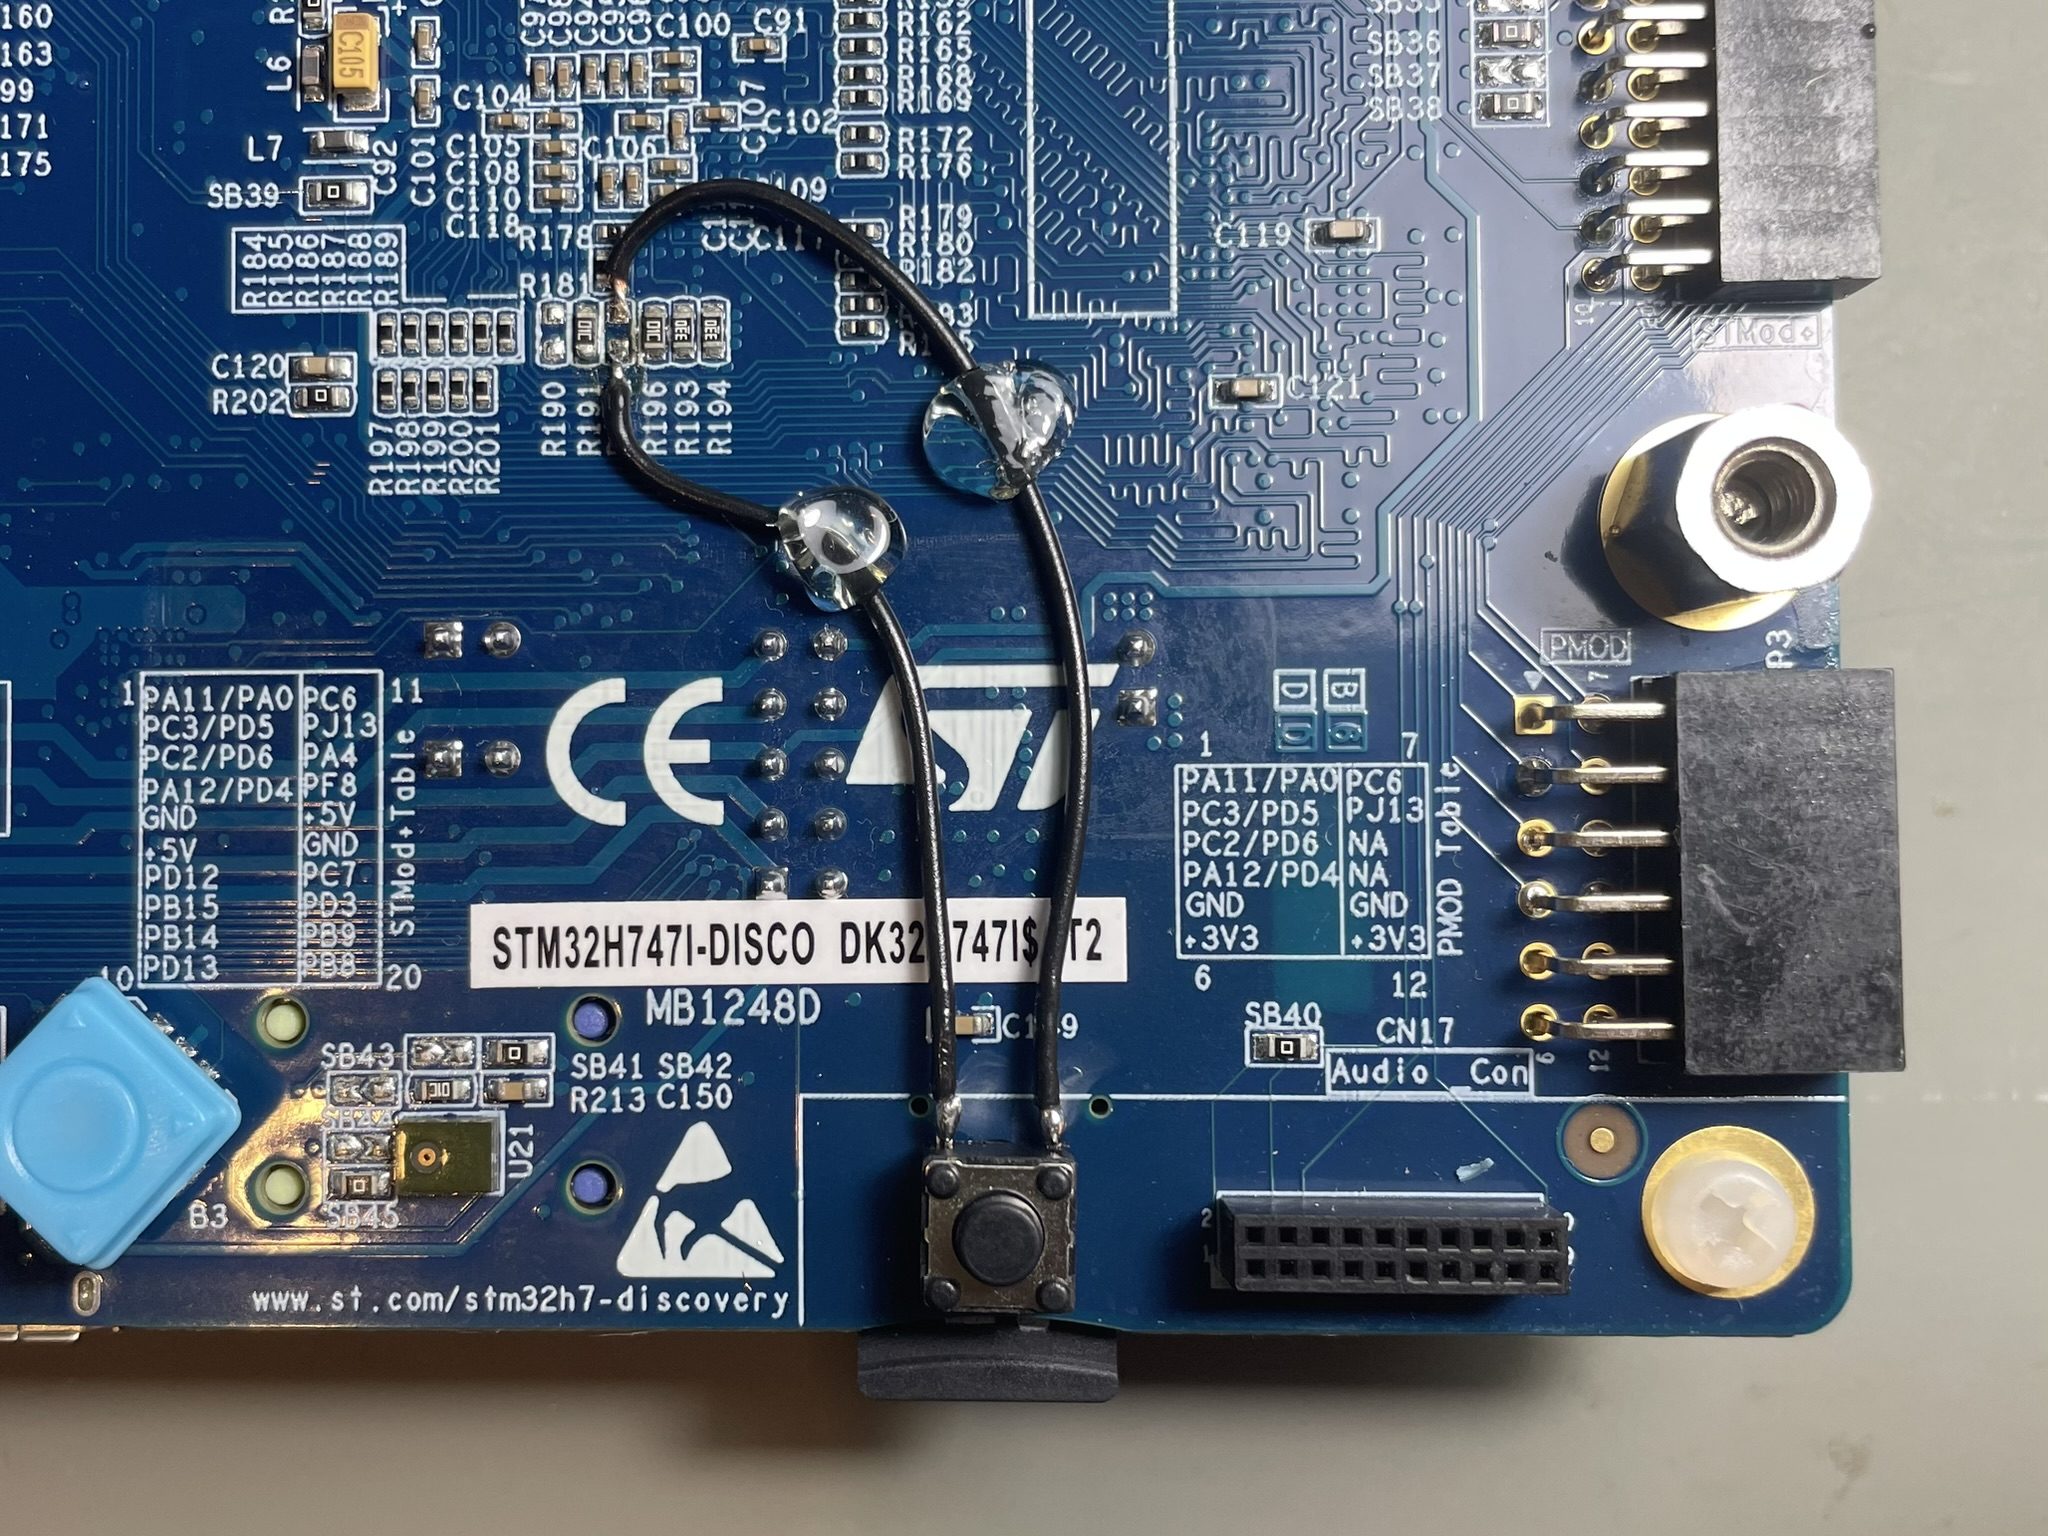
\includegraphics[width=10cm]{Resources/HW_Boot_MOD.JPEG}
	\caption{Hardware Boot Button Mod}
	\label{fig:Hardware Boot Button Mod}
\end{figure}

Later it turned out, that those problems came from a faulty RCC configuration. That's something I should investigate further. Because right now I'm only able to get up to 400MHz for the CM7. This probably has something to do with the SMPS and Voltage scaling option in the RCC tab.

\section{QSPI Flash}
To extend the internal flash of the MCU, there is 128MB of QSPI Flash on the DevBoard. In this section I'll try to implement this flash, so I'm able to store the actual firmware on this external flash. This also means, that the MCU should then boot from the external memory.

\subsection{Write Test}
In this first test I'll try to simply write some data to the Flash and therefore confirm, that the communication between the MCU and flash works as intended. For this I've again followed the instructions from Controllers Tech on YouTube. 
\cite{YT_CT_QSPI}

\begin{enumerate}
	\item Enable QSPI block in "Dual Bank with Quad Lines" mode (Because DevBoard uses two ICs, each 512Mbit) for CM7.
	\item Set up pins according to the schematics. (standard cube config is wrong.) Configure Pins to CM7 in "very high" speed mode.
	\item Enable chip select 1 for both banks.
	\item Set clock prescaler to 2. (200MHz Clock divided by 2 to the power of 2 \(\rightarrow\) 50MHz ) (Flashs max. frequency in DTR mode (dual bank) is 90MHz)
	\item Fifo threshold to 4.
	\item Sample shifting to "Sample Shifting Half Cycle"
	\item Flash size to 26. (Flash size is 2 to the power of 26 + 1 Bytes. \(\rightarrow\) 128MB )
	\item Chip select high time to "6 Cycles"
	\item For Cortex-M7 Enable: ICache and DCache.
	\item Generate code.
	\item Then add user code lines from STM GitHub. \cite{GIT_DRIVER_QSPI_FLASH} to qspi.c and qspi.h.
\end{enumerate}

Now you can download the firmware to the MCU. And verify, that no error is triggered. (Orange LED blinking) Then to verify, that the string was written to the flash: open STM32CubeProgrammer and enable the external loader for the H747-Disco DevBoard. Now at the address 0x90000000, the string "msgOut" should be shown.

\lstset{language=C,caption={QSPI Write Test CM7},label=DescriptiveLabel, style=mystyle}
\begin{codeblock}
	\lstinputlisting{../../../6_Software/qspi flash/CM7/Core/Usercode/usermain_CM7.c}
\end{codeblock}

While playing a bit with this code, I've noticed, that the flash can't manipulate single bits. It can just turn a 1 into a 0 but nor in reverse. To set a 0 to a 1 you have to erase a whole sector or the whole chip. After some research on this topic I've learned, that this behaviour is common for flash memories, as they're normally only used to store data over a long time. For example: Firmware.


\subsection{Boot from QSPI}
After trying to boot from the QSPI flash, I decided to change my plans an go on without a bootloader and external RAM. At the moment I don't know to less debug the problems I've had and therefore I decided to go on with the easier tasks of this project like the actual measurements and move the Memories implementation to another project.



\section{User Interface}
I first tried to use TouchGFX to design an embedded UI using STMs TouchGFX which is a code generator for graphical displays with STM32 microcontrollers. But it turned out, that it's a lot more complicated that I originally thought. This is due to the usage of FreeRTOS and C++, which I both didn't know by then. So also because of the limited time I decided to make a tkinter app in python to show the measured values. The app is in the software folder and has the name "CircuitVoyager UI". As a base I used the following GitHUB repo: \cite{Python_Serial_Port_Tkinter_GUI}
\chapter{Conclusion}
\label{cha:Conclusion}


\textbf{Project Start}

I've noticed that it was quite hard for me to start with the project. There are so much topics to imply, that it can get overwhelming and very emotional. I've also underestimated the time needed to set up the documentation LaTeX files and the whole planning. It can be demotivating if you're spending a lot of time and in the end didn't really start with the project. But later I was able to start the project without much trouble. 

\vspace{5mm}
\textbf{Time Plan}

Well, the GANTT chart as you can see didn't help out much for me. Because it's really hard to plan such a projects timing over half a year. There are so many unsolved problems and in the beginning I haven't been able to estimate the duration of all the processes involved. On the other hand my 2-week plans were working great and helped a lot, to notice what was to do.

\vspace{5mm}
\textbf{HW development}

I've learned much in this project part. Mainly this was Altium Designer, as this was my first complete project I've realized in Altium Designer. This also leaded to some not nicely solved solution. All components for example have their own properties and this leads to a unreadable BOM.

But in the end I've also noticed, that the dataflow (that usually should go from left to right) goes in the wrong direction. This had already started in the HW-Chart and therefore also ended up in the schematic.

I've also used Draw.io one of the first times and by now it looks very promising. It's much easier and more straight forward than MS Visio. Everything just works as intended.

\vspace{5mm}
\textbf{SW development}

Because in this project I've used a dual-core MCU for the first time, it was really hard to write the code at first. And with time I noticed that it's to complicated for me to implement such modern techniques. This is also due to the bad documentation of tools like FreeRTOS TouchGFX or multicore MCUs.

\newpage
\textbf{Project Idea}

The Project Idea in the first was really good. But as you can see, some minor decisions weren't as intelligent as they could be. I noticed that I'm much better at the "old style" electronics, without any operating system, overpowered MCUs, or TouchGFX. But I'm happy, that I was able to switch the focus of my project from hi-speed protocols to more embedded software and LaTeX. In the end I have a product that I'm proud of and that works. But I won't move on with the Circuit Voyager in the next semester, because I also noticed, that It's rather hard to make the hardware development of measurement equipment. This takes a lot of time, also away from school. And in the next semester I want to focus more on stuff like Swiss Skills and therefore make an easier project.

\vspace{5mm}
\textbf{Outlook}

As described in the project idea chapter. I want to stop the development of the Circuit Voyager and move on with an easier more embedded and hardware close project with simpler protocols and so on. But on the other hand I'll also document my further projects with LaTeX, because I got a lot faster, and it's more predictable than MS Word.
\chapter{Appendix}\label{cha:Appendix}

\section{Journal}\label{sec:Journal}
\begin{table}[H]
    \centering
    
\begin{tabular}{||c | c | c || c||} 
 \hline
 Date &  Location & Duration & Activity \\ [0.5ex] 
 \hline\hline
  01.09.2023 & TBZ & 1.5h & Selected and bought \acs{devboard} \\ 
 \hline
 08.09.2023 & TBZ & 2h & Tested \acs{devboard} with demos \\ 
 \hline
  08.09.2023 & TBZ & 0.5h & Noted first ideas for \acs{dmm} \\ 
 \hline
   15.09.2023 & TBZ & 1.5h & Written and signed Project Agreement [\ref{sec:Project Agreement}] \\ 
 \hline
    21.09.2023 & Home & 3h & Created documentation template \\ 
 \hline
    22.09.2023 & TBZ & 2h &  Started writing Journal [\ref{sec:Journal}]\\ 
 \hline
    24.09.2023 & Home & 1.5h &  Made GANTT chart [\ref{sec:GANTT Chart}]\\ 
 \hline
    27.09.2023 & Home & 2h & Written detailed planning and introduction \\ 
 \hline
    29.09.2023 & TBZ & 1.5h & Added mindmap, Lasten-, Pflichtenheft \\ 
 \hline
    06.10.2023 & TBZ & 1h & Started with block diagram (extension PCB) \\ 
 \hline
    20.10.2023 & ETH & 0.5h & Started Altium Project, Schematic template \\ 
 \hline
    23.10.2023 & ETH & 3h & HW Concept / documentation \\ 
 \hline
   23.10.2023 & ETH & 3h & Start schematic / documentation \\ 
 \hline
   25.10.2023 & Home & 2h & Schematic: Current Src, Volt div \\ 
 \hline
   26.10.2023 & ETH & 1.5h & Schematic: Current meas, ERC \\ 
 \hline
   26.10.2023 & Home & 1h & Schematic: Cleanup, Comments, DS Saves \\ 
 \hline
   26.10.2023 & Home & 1h & Documentation \& prepared Interview 1 \\ 
 \hline
  27.10.2023 & TBZ & 1.5h & Documentation: Started with schematic part \\ 
 \hline
  28.10.2023 & Home & 2h & Documentation: schematic parts \\ 
 \hline
  29.10.2023 & Home & 1h & Docu: schematic done, resources cleanup \\ 
 \hline
   29.10.2023 & Home & 0.5h & Layout: Outline, Placement start \\ 
 \hline
   31.10.2023 & Home & 1h & Layout: Placement Done \\ 
 \hline   
   01.11.2023 & Home & 1.5h & Layout: Routing Done \\ 
 \hline
  02.11.2023 & Home & 1h & Layout: Cleanup \& Export \\ 
 \hline
  03.11.2023 & TBZ & - & Interview 1: signed by mala \\ 
 \hline  
  03.11.2023 & TBZ & 1h & Pepared BOM for supplying \\ 
 \hline
  04.11.2023 & Home & 1h & Documentation: PCB, Reflection \\ 
 \hline

\end{tabular}
    \caption{Project Journal 1}\label{tab:Project Journal 1}
\end{table}

\newpage

\begin{table}[H]
  \centering
  
  \begin{tabular}{||c | c | c || c||} 
    \hline
    Date &  Location & Duration & Activity \\ [0.5ex] 
    \hline\hline
    05.11.2023 & Home & 0.5h & STM32 Multicore Debugging \\ 
    \hline
     05.11.2023 & Home & 1h & Documentation: STM32 Multicore Debug \\ 
    \hline
     05.11.2023 & Home & 1h & Boot problems / HW MOD \\ 
    \hline
    09.11.2023 & Home & 3h & Population of 2 Extension PCBs \\ 
    \hline
    11.11.2023 & Home & 0.5h & HW MOD of second DevBoard \\ 
    \hline
  \end{tabular}
  \caption{Project Journal 2}\label{tab:Project Journal 2}
\end{table}

\newpage



\section{Weekly plans}
\label{sec:Project Planning}

\subsection{KW39 \& 40}
\begin{itemize}
    \item Write introduction
    \item Planning: Cost, Tools, When, Why
    \item Create project diagram (learning process)
    \item ''Lastenheft''
    \item ''Pflichtenheft''
    \item Make a \acs{hw}-Digram for the Extension \acs{pcb}.
    \item Make the schematic of the Extension \acs{pcb}. 
    \begin{itemize}
        \item Part to measure voltage.
        \item Part to measure current.
        \item Part to measure continuity.
        \item Addressable LEDs.
    \end{itemize}
    \item Start with the Layout of the Extension \acs{pcb}.
    \item Reflection of the start of the project.
\end{itemize}




\subsection{KW41 \& 42}
Fall holidays. I planned to invest much time in the holidays, but it turned out that my plans changed, and I was busy.



\subsection{KW43 \& 44}
Mainly catching up.
\begin{itemize}
    \item Make a \acs{hw}-Digram for the Extension \acs{pcb}.
    \item Make the schematic of the Extension \acs{pcb}. 
    \begin{itemize}
        \item Part to measure voltage.
        \item Part to measure current.
        \item Part to measure continuity.
        \item Addressable LEDs.
    \end{itemize}
    \item Make the whole Layout of the Extension \acs{pcb}.
    \item Order the Extension PCB and the components.
    \item Reflection of the start of the project.
\end{itemize}
and maybe if the time is sufficient I could start with implementing the SDRAM and QSPI Flash.



\subsection{KW45 \& 46}
\begin{itemize}
  \item Populate and commission the extension PCB.
  \item Implement QSPI flash with bootloader.
  \item Implement external SDRAM.
  \item Implement touch display. (MIPI DSI, Touch)
\end{itemize}
and maybe if the time is sufficient I could start with learning TouchGFX.

\newpage



\section{GANTT Chart}
\label{sec:GANTT Chart}
\label{fig:GANTT Chart}
\begin{figure}[H]
	\centering
    \framebox{
	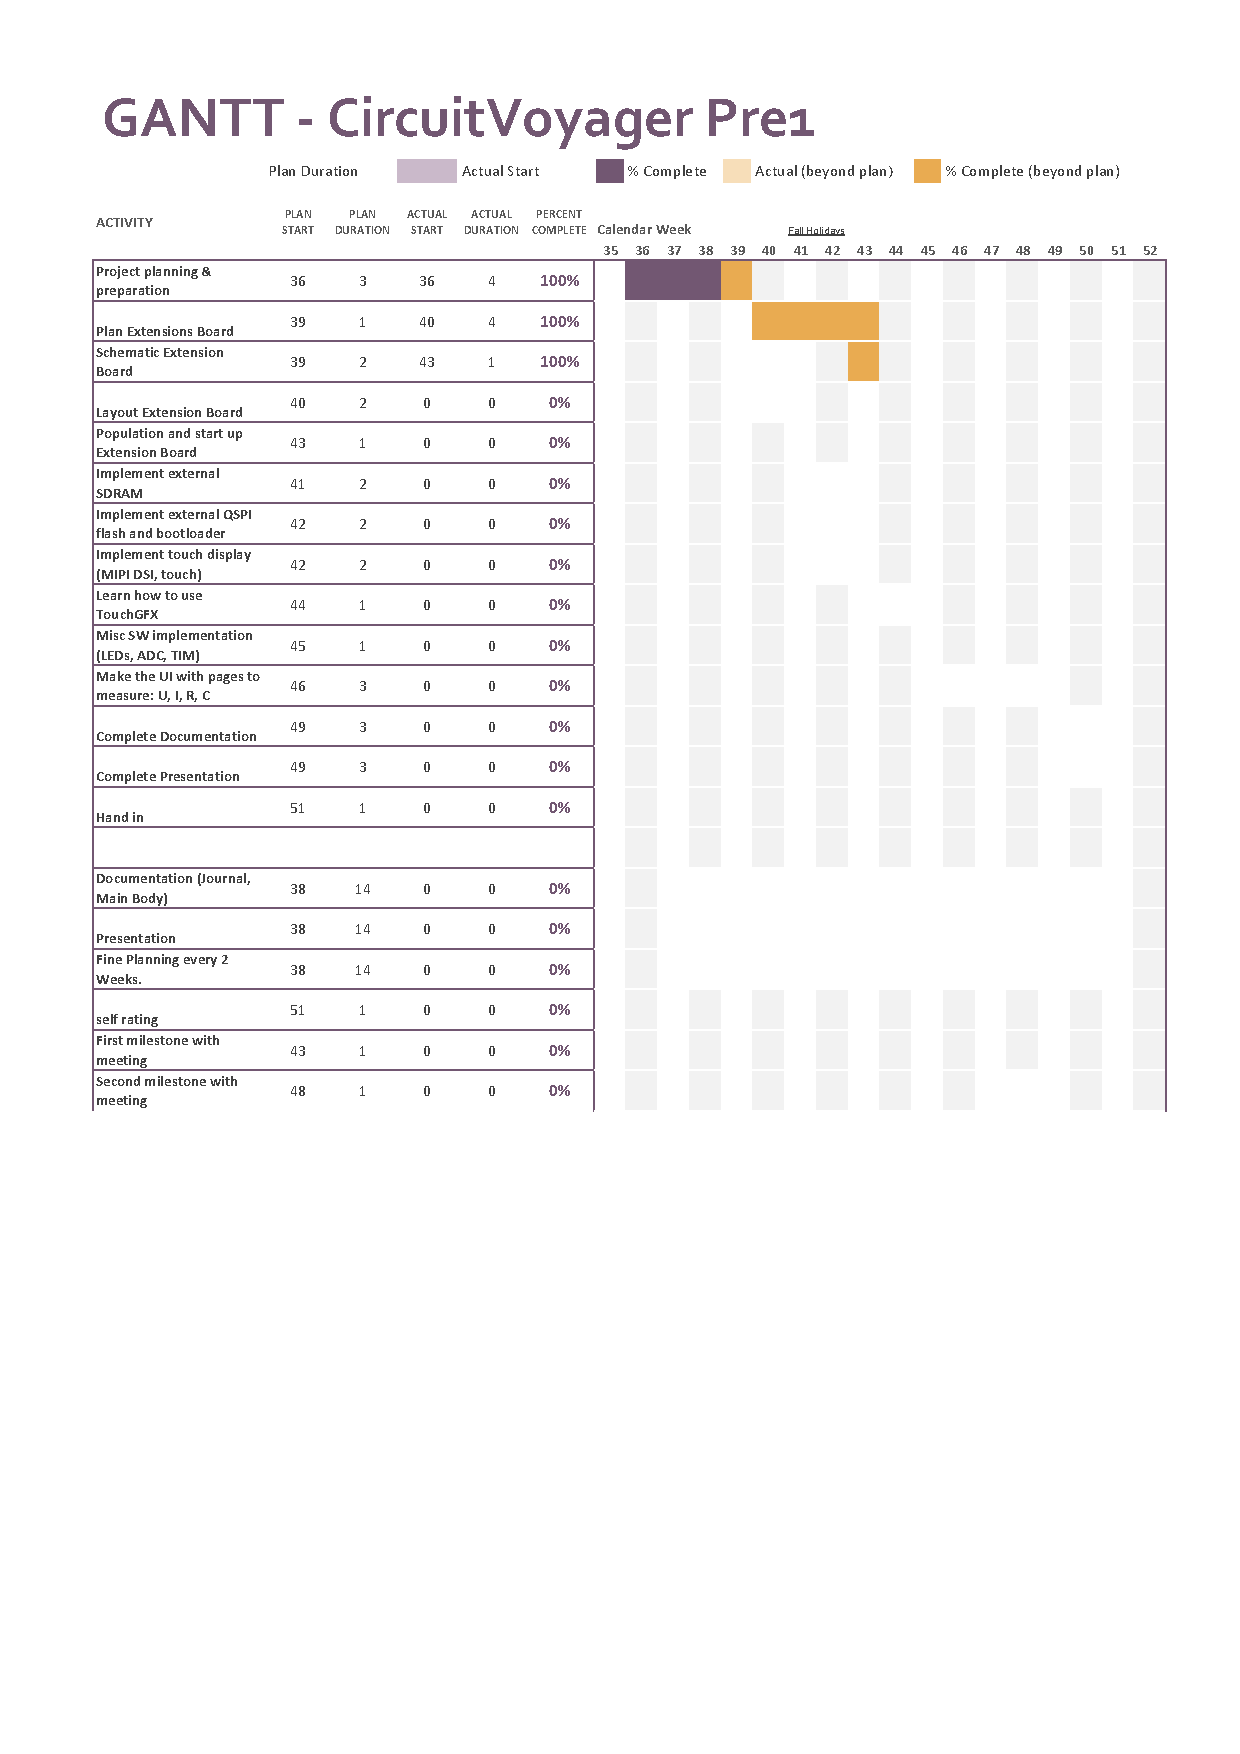
\includegraphics[width=14.5cm]{../../2_Project_Planning/GANTT/GANTT.pdf}}
	\caption{GANTT Chart}
\end{figure}
\newpage




\section{Project Agreement}
\label{sec:Project Agreement}
\begin{figure}[H]
  \label{fig:Project Agreement}
	\centering
    \framebox{
	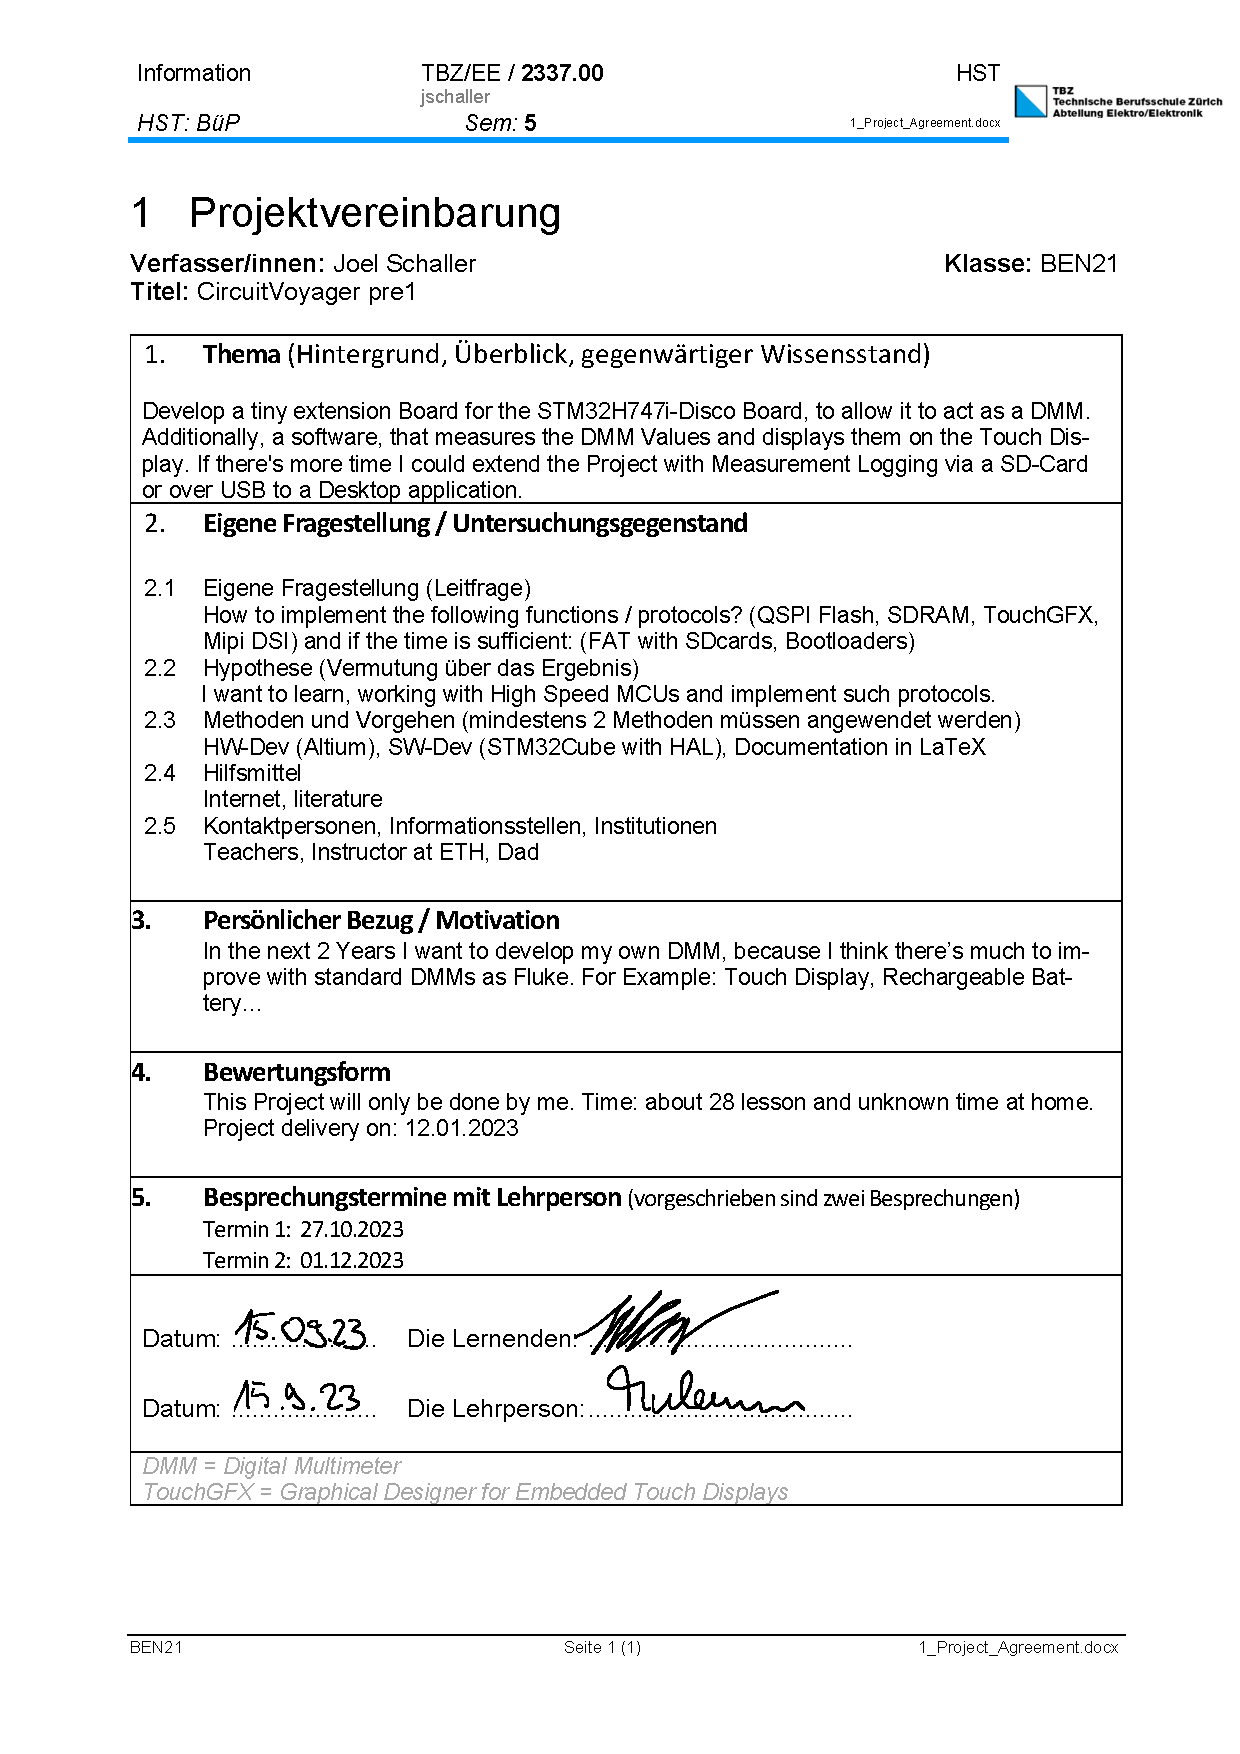
\includegraphics[width=14.5cm]{../../../1_Agreement_Review/1_Project_Agreement_CircuitVoyager_pre1_jschaller_230915.pdf}}
	\caption{Project Agreement}
\end{figure}
\newpage

\section{Interview 1}
\label{sec:Interview 1}
\begin{figure}[H]
  \label{fig:Interview 1}
	\centering
    \framebox{
	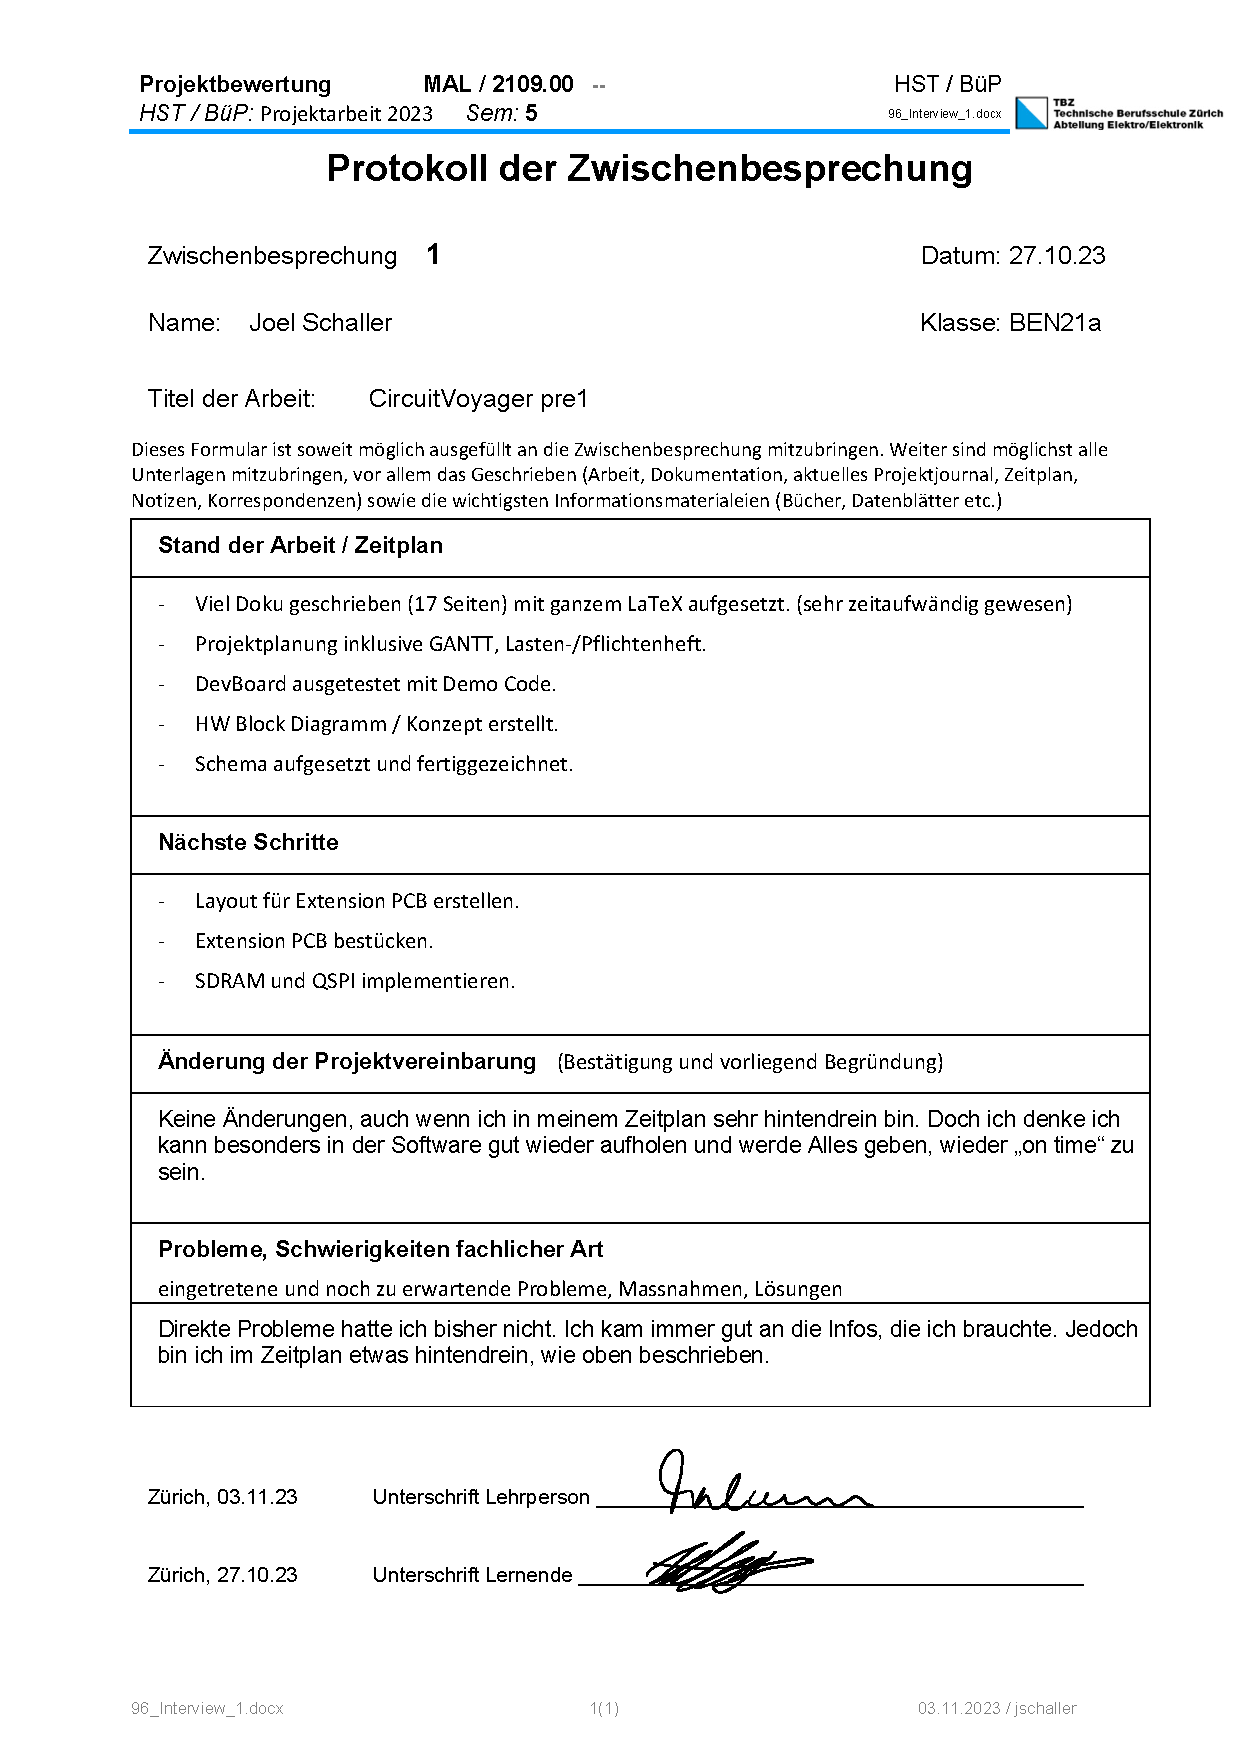
\includegraphics[width=14.5cm]{../../../1_Agreement_Review/96_Interview_1.pdf}}
	\caption{Interview 1}
\end{figure}
\newpage



\section{Extension PCB Schematics}
\label{sec:Extension PCB Schematics}
\begin{figure}[H]
	\centering
	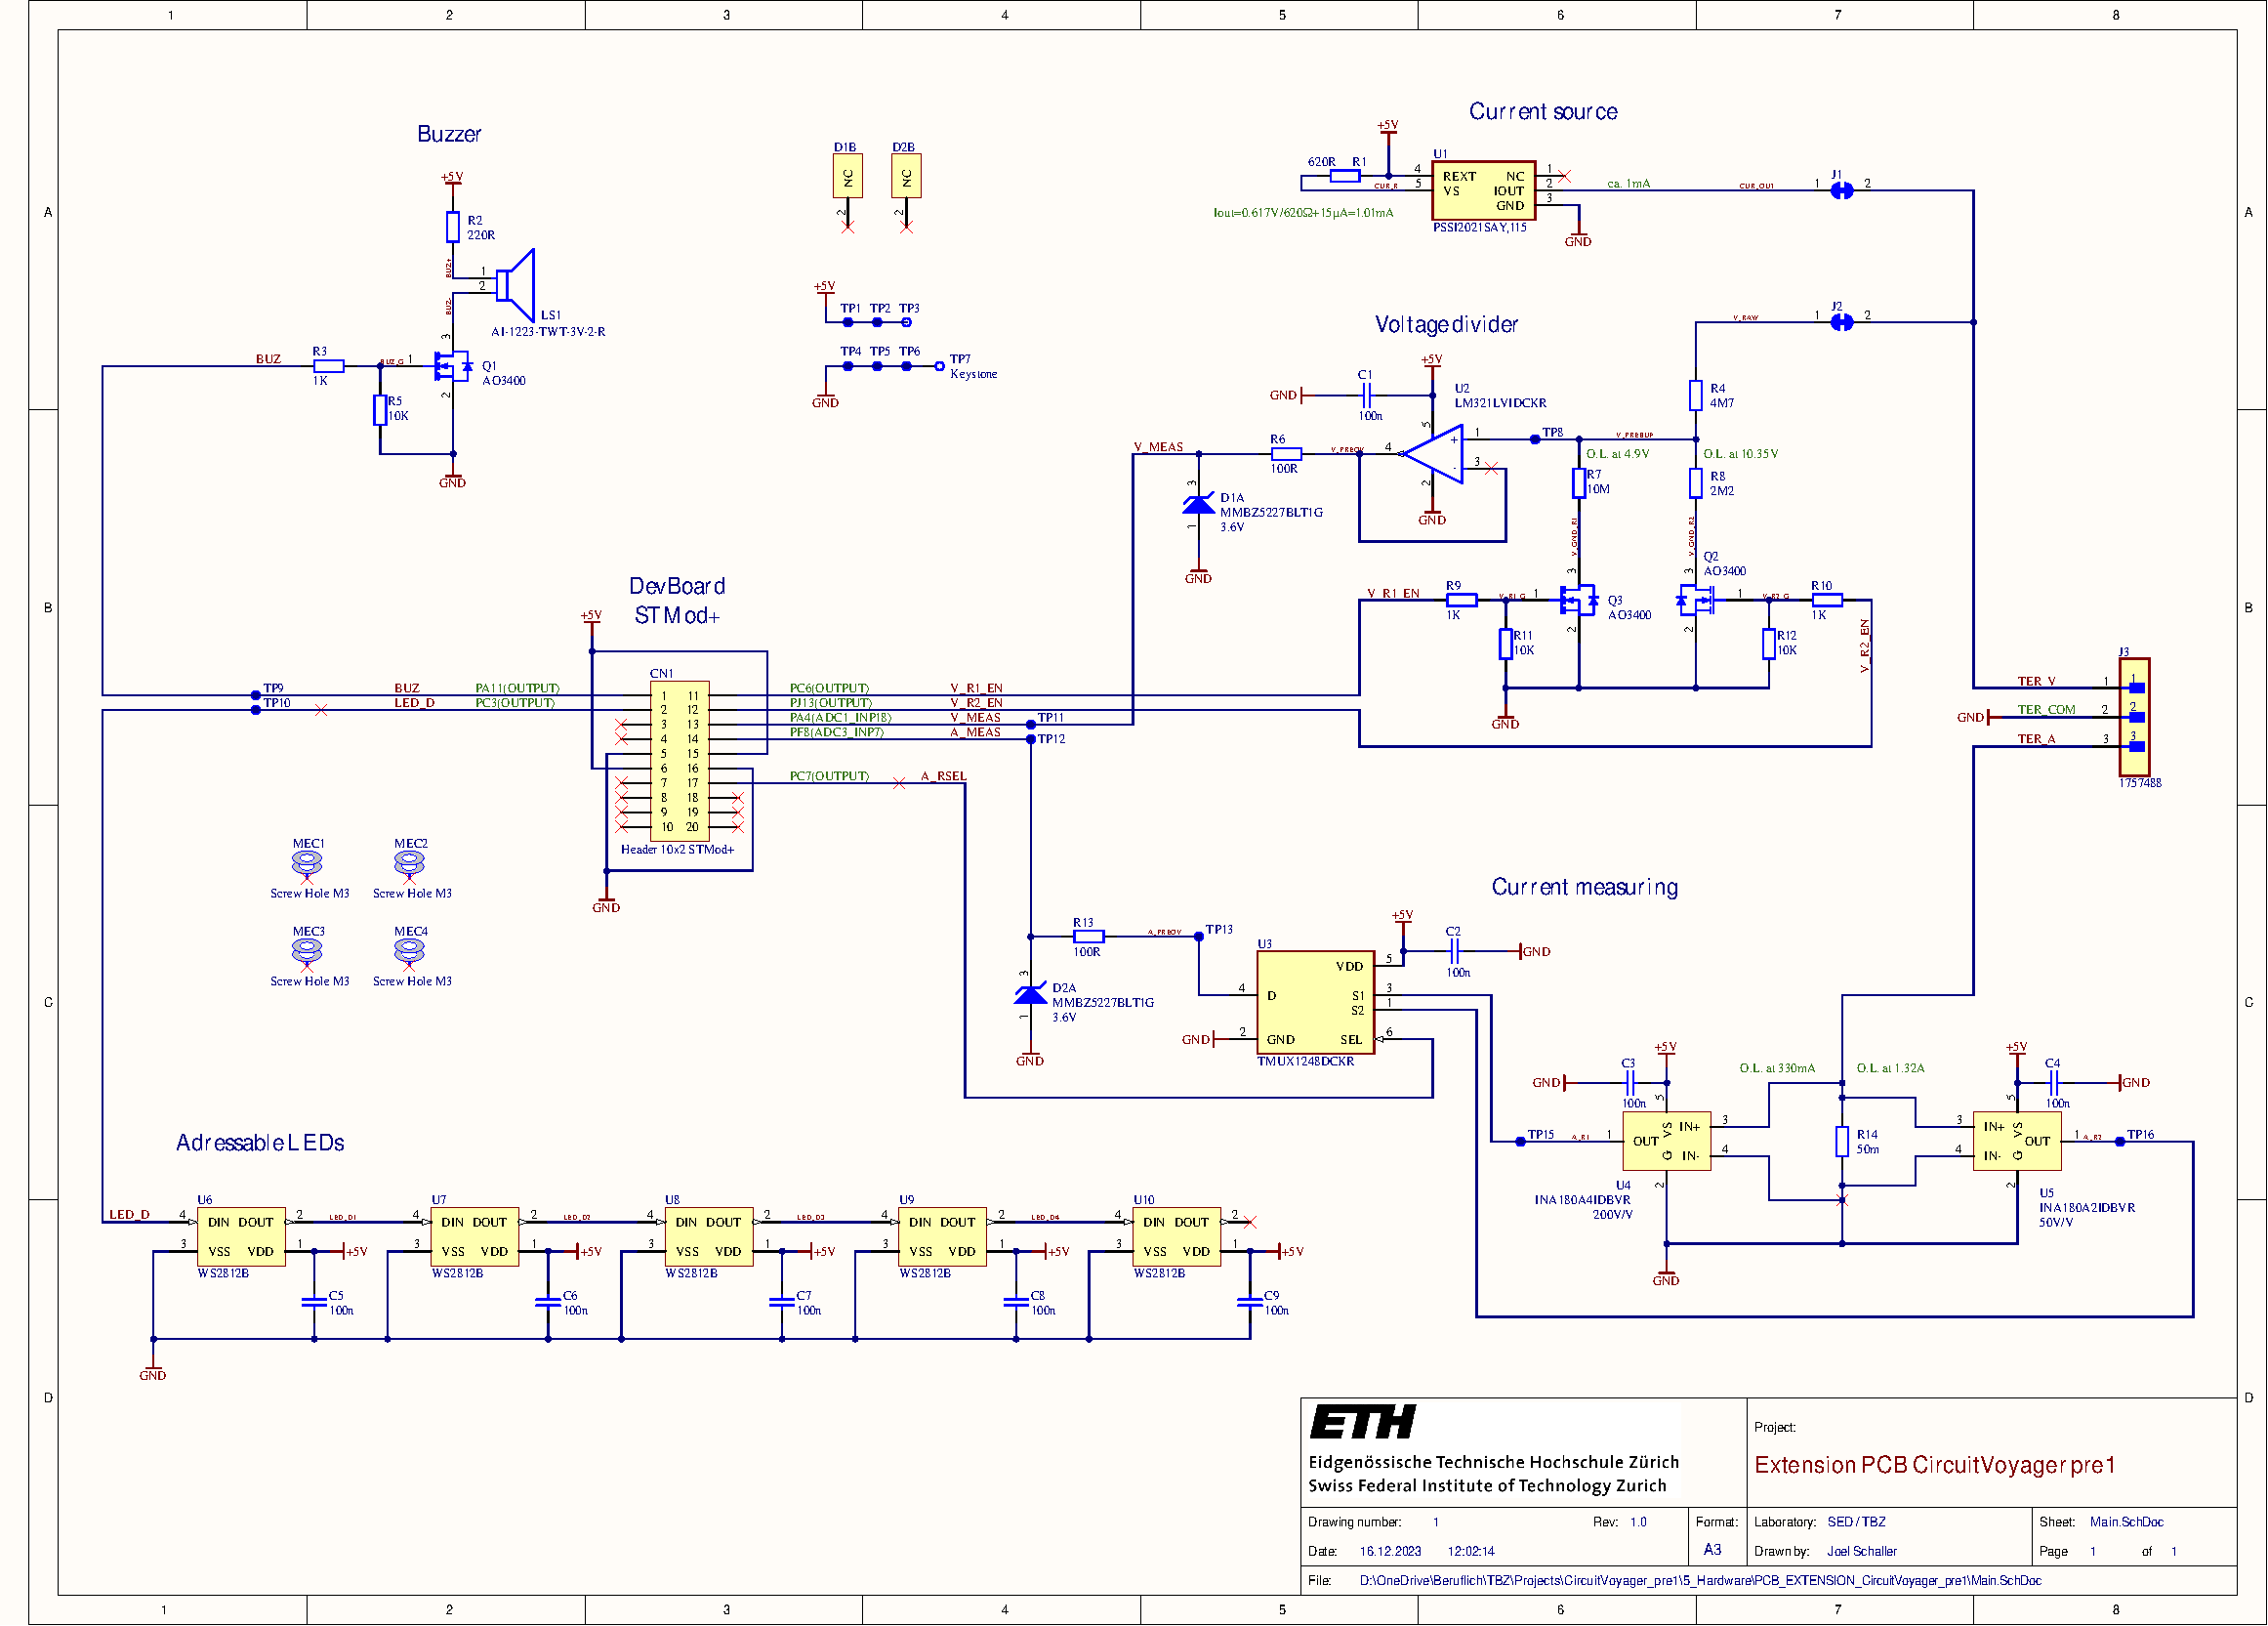
\includegraphics[height=15cm, angle=270]{../../../5_Hardware/PCB_EXTENSION_CircuitVoyager_pre1/Project Outputs for PCB_EXT_CV_PRE1/Schematic_PCB_EXTENSION_CircuitVoyager_pre1.pdf}
	\caption{Extension PCB Schematics}
	\label{fig:Extension PCB Schematics}
\end{figure}


\section{Extension PCB Manufacture 11.23 BOM}
\label{sec:Extension PCB Manufacture 11.23 BOM}
\begin{figure}[H]
	\centering
  \framebox{
	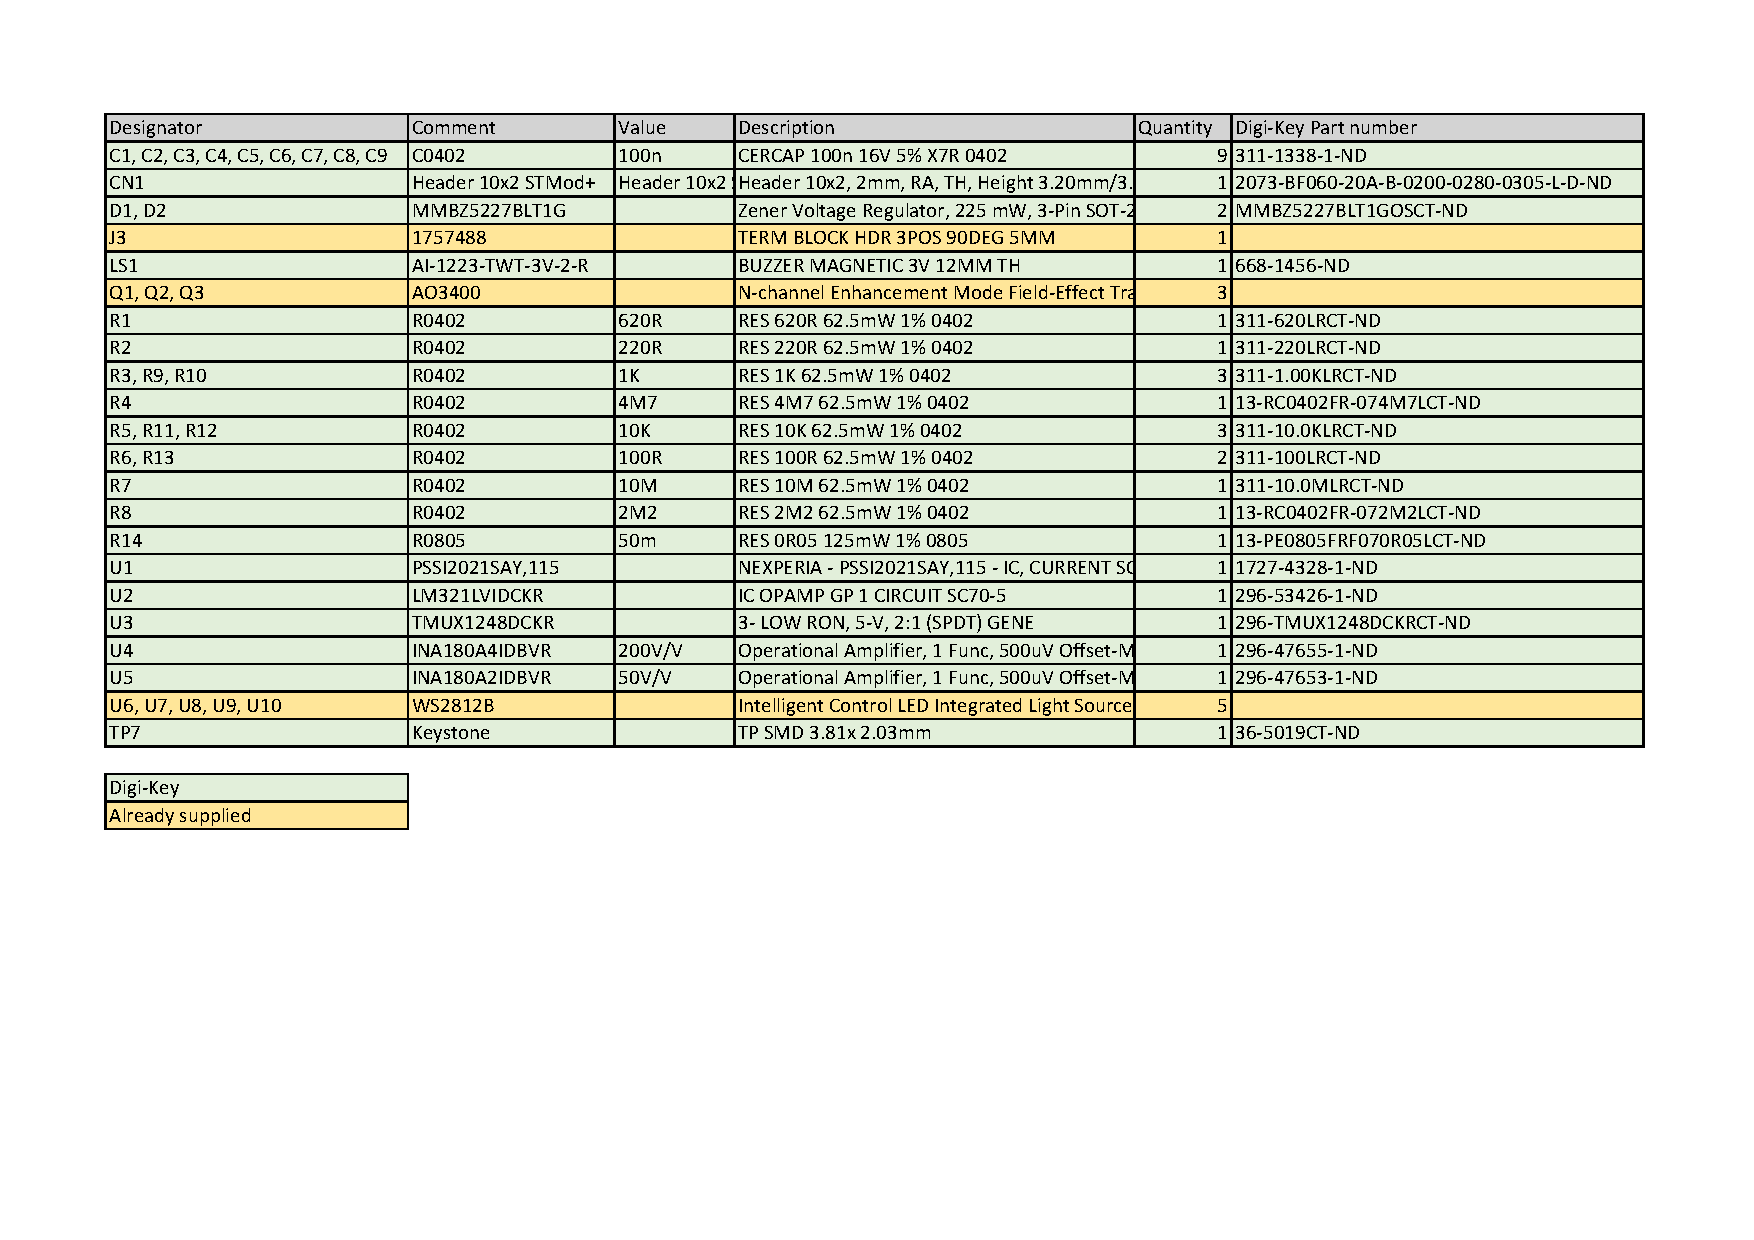
\includegraphics[height=14.5cm, angle=270]{../../../5_Hardware/PCB_EXTENSION_CircuitVoyager_pre1/MANUFACT_2311/BOM-PCB_EXT_CV_PRE1.pdf}
  }
	\caption{Extension PCB Manufacture 11.23 BOM}
	\label{fig:Extension PCB Manufacture 11.23 BOM}
\end{figure}
\newpage


\newpage

\pagestyle{icmt-fancy} 
% List of bibliography (displays cite elements)
\bibliography{Bibliography}
\addcontentsline{toc}{chapter}{\bibname}
\cleardoubleemptypage
%% List of figures
\listoffigures
\addcontentsline{toc}{chapter}{\listfigurename}
\cleardoubleemptypage
% List of tables
\listoftables
\addcontentsline{toc}{chapter}{\listtablename}
\cleardoubleemptypage
% List of code elements
\lstlistoflistings
\addcontentsline{toc}{chapter}{Listings}
\cleardoubleemptypage
\chapter*{Acronyms}
\begin{acronym}
        \acro{circuitvoyager}[CircuitVoyager]{The Name of the \acs{dmm} I'm developing.}
        \acro{devboard}[DevBoard]{main microcontroller developement board. (STM32H747I-Disco)}
        \acro{dmm}[DMM]{digital multimeter}
        \acro{hw}[HW]{Hardware}
        \acro{sw}[SW]{Software}
        \acro{qspi}[QPSI]{Quad \acs{spi}}
        \acro{spi}[SPI]{Serial Peripheral Interface (low level protocol)}
        \acro{sdram}[SDRAM]{Synchronous Dynamic Random Access Memory (external RAM)}
        \acro{touchgfx}[TouchGFX]{Graphical \acs{ui} designer for STM32 \acs{mcu}s}
        \acro{ui}[UI]{User Interface}
        \acro{mcu}[MCU]{Micro Controlling Unit}
        \acro{mipidsi}[Mipi DSI]{Digital Serial Interface (Display Protocol)}
        \acro{fat}[FAT]{File Allocation System (Low Level Filesystem)}
        \acro{hal}[HAL]{Hardware Abstraction Layer (STM32 Abstraction Library)}
        \acro{ethz}[ETHZ]{Eidgenössische Technische Hochschule}
        \acro{tbz}[TBZ]{Technische Berufsschule Zürich}
        \acro{adc}[ADC]{Analog Digital Converter}
        \acro{tim}[TIM]{Timer (Hardware Block in STM32)}
        \acro{pcb}[PCB]{Printed Circuit Board}
        \acro{dut}[DUT]{Device under test}
        \acro{ovp}[OVP]{Over voltage protection}
\end{acronym}
\addcontentsline{toc}{chapter}{Acronyms}

\end{document}
% ============= End of the main document =============
